\documentclass[11pt,a4paper]{article}

\usepackage[utf8]{inputenc}
\usepackage[T1]{fontenc}
\usepackage[english]{babel}
\usepackage[a4paper,margin=2.4cm]{geometry}

\usepackage{amsmath, amssymb, amsthm}
\usepackage{mathtools}
\usepackage{booktabs}
\usepackage{tabularx}
\usepackage{array}
\usepackage{caption}
\usepackage{float}
\usepackage{enumitem}
\usepackage{microtype}
\usepackage{xcolor}
\usepackage{listings}
\usepackage{fancyhdr}
\usepackage{titlesec}
\usepackage{graphicx}
\usepackage{tikz}
\usetikzlibrary{positioning, arrows.meta, fit, backgrounds, calc, shapes.geometric}
\usepackage[hidelinks]{hyperref}

%  ---  Palette shared with the companion reports  ---
\definecolor{ink}{RGB}{26,30,36}
\definecolor{slate}{RGB}{92,101,112}
\definecolor{mist}{RGB}{233,235,238}
\definecolor{rulegrey}{RGB}{188,194,201}
\definecolor{steel}{RGB}{47,72,102}
\definecolor{steellight}{RGB}{124,146,172}
\definecolor{signal}{RGB}{160,32,45}

\hypersetup{
    colorlinks=true,
    linkcolor=steel,
    citecolor=steel,
    urlcolor=steel,
    pdftitle={Contamination with a Location: A Three-Site Epistemic Survey Executed by Two Robots under Open-RMF},
    pdfauthor={Haniel Ulises},
}

\color{ink}

\setlength{\headheight}{22pt}
\pagestyle{fancy}
\fancyhf{}
\fancyhead[L]{\small\textcolor{slate}{\itshape Contamination with a Location}}
\fancyhead[R]{\small\textcolor{slate}{\thepage}}
\renewcommand{\headrulewidth}{0.4pt}
\renewcommand{\headrule}{\hbox to\headwidth{\color{rulegrey}\leaders\hrule height \headrulewidth\hfill}}

\titleformat{\section}{\normalfont\large\bfseries\color{ink}}{\thesection}{0.7em}{}
\titleformat{\subsection}{\normalfont\normalsize\bfseries\color{ink}}{\thesubsection}{0.7em}{}
\titleformat{\paragraph}[runin]{\normalfont\bfseries\color{slate}}{}{0em}{}[.]

\captionsetup{font=small, labelfont={bf,color=slate}, textfont=footnotesize}

\theoremstyle{definition}
\newtheorem{definition}{Definition}
\newtheorem{proposition}{Proposition}

\lstdefinestyle{sys}{
    backgroundcolor=\color{mist},
    basicstyle=\ttfamily\scriptsize\color{ink},
    keywordstyle=\color{steel}\bfseries,
    commentstyle=\color{slate}\itshape,
    stringstyle=\color{slate},
    morecomment=[l]{\#},
    % Deliberately short. Most of the listings here are log excerpts, and
    % colouring their ordinary nouns marks a transcript as though it were
    % source. Only the declarations of the domain are highlighted.
    morekeywords={:types,:predicates,:objects,:agents,:goal,:init,site,agent},
    frame=single,
    rulecolor=\color{rulegrey},
    framesep=5pt,
    xleftmargin=6pt,
    xrightmargin=0pt,
    breaklines=true,
    showstringspaces=false,
    columns=fullflexible,
    captionpos=b,
}
\lstset{style=sys}

%  ---  Notation  ---
\newcommand{\Ag}{\mathcal{A}}
\newcommand{\Mod}{\mathcal{M}}
\newcommand{\Ev}{\mathcal{E}}
\newcommand{\prd}{\otimes}
\newcommand{\Kop}[1]{K_{#1}}
\newcommand{\Kw}[1]{\mathit{Kw}_{#1}}
\newcommand{\code}[1]{\texttt{\small #1}}
\newcommand{\site}[1]{\code{#1}}

\begin{document}

\begin{titlepage}
\centering
\vspace*{2.4cm}
{\color{rulegrey}\rule{\textwidth}{0.8pt}}\\[0.9cm]
{\LARGE\bfseries Contamination with a Location\par}
\vspace{0.5cm}
{\large\color{slate} A Three-Site Epistemic Survey Executed by Two Robots\\ under Open-RMF, and a Correction to the Floor\par}
\vspace{0.7cm}
{\color{rulegrey}\rule{\textwidth}{0.8pt}}\\[1.4cm]

{\large Haniel Ulises\par}
\vspace{0.3cm}
{\color{slate} Epistemic Robotics}\\
\vspace{0.15cm}
{\color{slate}\today}

\vfill
{\color{slate}\small
The companion report executes an epistemic policy over forty metres of
warehouse and states, at its outset, that floor area and epistemic difficulty
are independent quantities. That statement is exact, and it is structural: the
proposition under uncertainty carries no argument, one site exists, and the
planner is therefore indifferent to geometry. This report removes the
independence by giving contamination a location. Exactly one of three sites is
contaminated; which one is unknown to every agent. The change is one line of
\textsc{epddl}. It multiplies the search by four orders of magnitude, doubles
the policy, and sends two robots to two aisles. Its principal consequence is
epistemic: on one branch the team terminates in possession of the state of a
site that no robot approached and no sensor observed.

\vspace{0.6em}
A second result is negative and concerns the floor of the companion report. The
world file carries a saved state block which the simulator applies in
preference to the poses the models declare. The two disagree for fourteen
models. The navigation graph of the companion report was therefore derived from
a building the simulator does not load, and its published figures are
superseded by those given here.}
\vspace{1.2cm}
\end{titlepage}

\tableofcontents
\newpage

%  ======================================================================
\section{Scope}
\label{sec:scope}

This report concerns a single modification to a previously reported epistemic
survey domain, and the consequences of that modification for search, for
execution, and for the derivation of the floor the execution takes place on.

The modification is the introduction of a type. Where the companion domain
declares the propositional atom $\mathit{contaminated}$, this domain declares
the predicate $\mathit{contaminated}(s)$ over a type $\mathit{site}$, together
with the common-knowledge constraint that exactly one site of three satisfies
it. Every other component is held fixed: three agents, an $\mathrm{S5}_3$
frame, one semi-private sensing action, two private announcement actions, and a
goal of the same form.

Three claims are advanced, and each is bounded in
Section~\ref{sec:established}.

\begin{enumerate}[leftmargin=1.4em, itemsep=2pt]
  \item A team of agents terminated in possession of knowledge concerning a
        location that no member visited and no sensor measured, obtained by
        elimination, with the negative conjunct of the goal intact over that
        location.
  \item Two robots each contributed one measurement, at sites separated by
        \(33.7\)\,m on a roadmap derived from the world, with transit costs of
        \(36.5\) and \(26.8\)\,m from their respective chargers.
  \item One policy traversed three distinct leaves in three worlds differing by
        the position of a single object, and satisfied its goal on each.
\end{enumerate}

Four bounds are stated at the outset, since they qualify everything that
follows. The nine scripted pedestrians in the world are scenery: they are
absent from the navigation graph and are neither perceived nor avoided. The
private channel is realised by topic addressing, which establishes that the
excluded agent was not addressed and does not establish that it could not have
listened. The executor traverses a policy in strict order, so the two robots
act sequentially and no claim of concurrency is made. Finally, the corrected
floor of Section~\ref{sec:floor} is established to be a correction; it is not
established that no further discrepancy of the same kind remains in the world
file.

%  ======================================================================
\section{Preliminaries}
\label{sec:prelim}

The vocabulary of this report is that of dynamic epistemic logic. It is
restated here in the form the implementation uses, because two of the
measurements reported below are of quantities the definitions introduce: the
cardinality of a model after a product update, and the partition an agent's
accessibility relation induces.

\subsection{Models}

\begin{definition}[Epistemic model]
\label{def:model}
Let $\Ag$ be a finite set of agents and $P$ a finite set of atomic
propositions. An \emph{epistemic model} is a tuple
$\Mod = (W,\, R,\, V,\, W_d)$ in which $W$ is a finite non-empty set of
\emph{worlds}; $R : \Ag \to 2^{W \times W}$ assigns to each agent an
\emph{accessibility relation}; $V : W \to 2^{P}$ assigns to each world the
atoms true at it; and $\emptyset \neq W_d \subseteq W$ is the set of
\emph{designated} worlds.
\end{definition}

A model is \emph{pointed} when $|W_d| = 1$ and \emph{multi-pointed} otherwise.
The designated set is the model's account of which worlds may be the actual
one; a multi-pointed model is therefore the representation of an initial
situation under uncertainty, and the reduction of $|W_d|$ over the course of a
run is the acquisition of knowledge by the system as a whole.

The frame here is $\mathrm{S5}_n$: each $R(a)$ is an equivalence relation, and
$\Ag = \{\mathit{scout},\, \mathit{relay},\, \mathit{observer}\}$, so $n = 3$.
Two consequences are used below. Each $R(a)$ partitions $W$ into equivalence
classes, and that partition is a complete description of the relation; and
knowledge is veridical, so an agent may be ignorant and cannot be mistaken.

\begin{definition}[Satisfaction]
\label{def:sat}
For $w \in W$, satisfaction of the modal fragment is
\[
  \Mod, w \models \Kop{a}\varphi
  \quad\text{iff}\quad
  \Mod, v \models \varphi \ \text{ for every } v \text{ with } (w,v) \in R(a),
\]
with the Boolean cases as usual. \emph{Knowing whether} abbreviates
$\Kw{a}\varphi \;\equiv\; \Kop{a}\varphi \vee \Kop{a}\neg\varphi$. A formula
holds at $\Mod$ when it holds at every designated world.
\end{definition}

The goals of Section~\ref{sec:domain} are stated in terms of $\Kw{a}$ and its
negation, and not of $\Kop{a}$. The distinction is material. $\Kw{a}\varphi$ is
satisfied by an agent that has settled the question either way, and a goal
demanding $\Kop{a}\varphi$ would require the world to be one in which $\varphi$
holds, which is a demand on the environment and not on the agent.

\subsection{Events and product update}

\begin{definition}[Event model]
\label{def:event}
An \emph{event model} is a tuple $\Ev = (E,\, Q,\, \mathit{pre},\,
\mathit{post},\, E_d)$ in which $E$ is a finite non-empty set of \emph{events};
$Q : \Ag \to 2^{E \times E}$ assigns to each agent an accessibility relation
over events; $\mathit{pre} : E \to \mathcal{L}$ assigns to each event a
precondition; $\mathit{post} : E \to (P \rightharpoonup \{\top,\bot\})$ assigns
a partial valuation change; and $E_d \subseteq E$ is the set of designated
events.
\end{definition}

The relation $Q(a)$ is the formal content of an action's
\emph{observability condition}. An agent for which $Q(a)$ is the identity on
$E$ distinguishes every event and therefore observes the action fully; an agent
for which $Q(a)$ is the total relation $E \times E$ distinguishes none and
therefore observes only that some event of $\Ev$ occurred.

\begin{definition}[Product update]
\label{def:product}
The result of executing $\Ev$ in $\Mod$ is
$\Mod \prd \Ev = (W',\, R',\, V',\, W'_d)$ with
\begin{align*}
  W'    &= \{\,(w,e) \in W \times E \;:\; \Mod, w \models \mathit{pre}(e)\,\},\\
  R'(a) &= \{\,((w,e),(v,f)) \;:\; (w,v) \in R(a) \text{ and }
             (e,f) \in Q(a)\,\},\\
  V'((w,e)) &= \big(V(w) \setminus \mathit{post}(e)^{-}\big)
               \cup \mathit{post}(e)^{+},\\
  W'_d  &= \{\,(w,e) \in W' \;:\; w \in W_d \text{ and } e \in E_d\,\},
\end{align*}
where $\mathit{post}(e)^{+}$ and $\mathit{post}(e)^{-}$ are the atoms the event
sets true and false respectively.
\end{definition}

\begin{proposition}[Size bound]
\label{prop:bound}
$|W'| \le |W| \cdot |E|$, with equality exactly when every event's
precondition is satisfied at every world.
\end{proposition}

Proposition~\ref{prop:bound} is the quantity Table~\ref{tab:contraction}
measures against. Two mechanisms reduce $|W'|$ below the bound: a precondition
that fails at some world removes the corresponding pair, and the implementation
contracts the result under bisimulation, which merges worlds that no formula
distinguishes. The observed counts are therefore an upper bound on the
information the model carries and a lower bound on nothing.

\subsection{The three action types of the domain}

The domain declares three action types, and each is an event model of the form
above. Their observability conditions are what separates them;
Table~\ref{tab:actiontypes} states them.

\begin{table}[H]
\centering\small
\caption{The action types of the domain, as event models. $\mathrm{id}$ denotes
the identity relation on $E$ and $E^2$ the total relation. The final column is
the bound of Proposition~\ref{prop:bound}.}
\label{tab:actiontypes}
\begin{tabularx}{\textwidth}{@{}llXl@{}}
\toprule
\textbf{Type} & $|E|$ & \textbf{Observability} & \textbf{Bound} \\
\midrule
public ontic
  & 1
  & $Q(a) = \mathrm{id}$ for every $a \in \Ag$. Every agent observes the event,
    and no agent's uncertainty is altered.
  & $|W|$ \\
\addlinespace
semi-private sensing
  & 2
  & $Q(i) = \mathrm{id}$ for the sensing agent $i$; $Q(a) = E^2$ for every
    other $a$. The performer distinguishes the two outcomes; the others learn
    that a sensing action occurred and not what it returned.
  & $2|W|$ \\
\addlinespace
private announcement
  & 2
  & $Q(i) = Q(j) = \mathrm{id}$ for speaker $i$ and listener $j$;
    $Q(a) = E^2$ for every other $a$. The second event is $\mathit{nil}$, with
    precondition $\top$ and no postcondition: it is the possibility, retained
    by every agent outside the audience, that nothing was said.
  & $2|W|$ \\
\bottomrule
\end{tabularx}
\end{table}

The $\mathit{nil}$ event is the formal reason a private announcement enlarges
the model. An agent outside the audience relates the announcement event to
$\mathit{nil}$, and therefore continues to consider possible a world in which
the utterance did not occur. The two directions of Section~\ref{sec:updates}
follow from the table without further argument: sensing constrains $W'_d$
through $E_d$ and leaves $|W|$ bounded by $2|W|$, while announcement leaves
$W'_d$ determined by one designated event and enlarges $W$.

%  ======================================================================
\section{The domain, and the cost of one argument}
\label{sec:domain}

\subsection{Formulation}

The domain is stated in \textsc{epddl} over a type $\mathit{site}$:

\begin{lstlisting}
(:types site)
(:predicates
  (contaminated ?s - site)
  (on-site ?i - agent ?s - site))
\end{lstlisting}

\noindent
The initial state asserts, as common knowledge among the three agents, that
exactly one of the three sites is contaminated, and that no agent knows which:

\[
  \Kop{C}\!\!\bigvee_{s \in S}\Big(
      \mathit{contaminated}(s) \wedge
      \bigwedge_{t \neq s} \neg\,\mathit{contaminated}(t)\Big),
  \qquad
  \Kop{C}\!\!\bigwedge_{i \in \Ag}\bigwedge_{s \in S}
      \neg\,\Kw{i}\,\mathit{contaminated}(s).
\]

The model therefore carries one world per site, all three designated. The goal
requires the scout and the relay each to come to know, for every site, whether
that site is contaminated, and requires the observer not to:

\[
  \bigwedge_{s \in S}\Kw{\mathit{scout}}\,\mathit{contaminated}(s)
  \;\wedge\;
  \bigwedge_{s \in S}\Kw{\mathit{relay}}\,\mathit{contaminated}(s)
  \;\wedge\;
  \bigwedge_{s \in S}\neg\,\Kw{\mathit{observer}}\,\mathit{contaminated}(s).
\]

Under the exactly-one constraint the first two conjunctions are satisfied by
settling any two sites, since the third is then determined. That implication is
the substance of the domain and is exploited by the policy of
Section~\ref{sec:policy}.

The goal is written as nine explicit conjuncts. The grounder rejects
\code{:forall} within a goal formula, and the quantified form is therefore
expanded at generation time.

\subsection{The cost of the argument}

Table~\ref{tab:scaling} records the grounded task and the search for the
propositional domain and for $k$ sites, $k \in \{2,3,4\}$. All rows were
grounded with \code{plank} and solved by \code{plansys2/Epistemic\-Plan\-Solver}
under \code{strategy=aostar} with the \code{ks} heuristic, three agents
throughout, on one machine.

\begin{table}[H]
\centering\small
\caption{Grounded task and search, as a function of the number of sites.}
\label{tab:scaling}
\begin{tabular}{@{}lrrrrrr@{}}
\toprule
\textbf{Domain} & \textbf{Atoms} & \textbf{Worlds} & \textbf{Actions}
  & \textbf{Depth} & \textbf{Expanded} & \textbf{Nodes} \\
\midrule
propositional      &  4 & 2 & 30 & 3 & 40      & 4 \\
$k = 2$ sites      &  8 & 2 & 48 & 3 & 147     & 4 \\
$k = 3$ sites      & 12 & 3 & 72 & 6 & 838\,168 & 8 \\
$k = 4$ sites      & 16 & 4 & 96 & \multicolumn{3}{c}{not solved within 901\,s} \\
\bottomrule
\end{tabular}
\end{table}

Three observations follow from the table.

\paragraph{The growth is not in the task} The grounded task grows linearly in
$k$: atoms, worlds and ground actions are $4k$, $k$ and $24k$ respectively. The
search does not. Expansion counts stand in the ratio $1 : 3.7 : 5\,702$ across
the first three rows, and the plan acquires four further actions between the
second row and the third.

\paragraph{Four sites is bounded, not refuted} Under the solver's default
fifteen-second budget the search reports \code{Timeout at depth 7}; under a
budget of nine hundred seconds it reports \code{Timeout at depth 8} after
$901$\,s and returns no plan. Both outcomes are exhaustion of the budget. No
claim is made here that $k = 4$ admits no solution. What is measured is the
price of the fourth site: a sixtyfold increase in budget purchased one
additional depth iteration.

\paragraph{The three-site search is fast and is nonetheless a hazard} The
planner logs the beginning of the search and the solution $6.4$\,s apart, so
$838\,168$ expansions correspond to approximately $1.3 \times 10^{5}$
expansions per second. That figure is not offered as a property of the search.
It is the proximate cause of the first defect of Section~\ref{sec:defects}: the
planner and the lifecycle manager of the planning system are served by one
executor in one process, and six seconds of uninterrupted search is sufficient
to starve the latter.

%  ======================================================================
\section{The plan}
\label{sec:policy}

The solver returns the eight-node conditional plan of
Figure~\ref{fig:policy}, at depth $6$ with three leaves.

\begin{figure}[H]
\centering
\begin{tikzpicture}[
  x=1mm, y=1mm,
  act/.style={draw=ink, fill=mist, rounded corners=2pt, inner sep=3.5pt,
              font=\ttfamily\scriptsize, align=center, minimum width=40mm,
              minimum height=6.5mm},
  sen/.style={act, draw=signal},
  ev/.style={->, >=Latex, draw=signal, thick},
  seq/.style={->, >=Latex, draw=slate},
  lab/.style={font=\ttfamily\tiny, text=signal, inner sep=1pt},
  leaf/.style={font=\scriptsize\itshape, text=slate}]

  \node[act] (g1) at (  0,   0) {goto relay a06};
  \node[act] (g2) at (  0, -13) {goto scout a17};
  \node[sen] (s1) at (  0, -26) {scan scout a17};
  \node[act] (r1) at (-55, -45) {relay scout relay a06};
  \node[act] (r2) at ( 55, -45) {relay scout relay a17};
  \node[sen] (s2) at ( 55, -58) {scan relay a06};
  \node[act] (r3) at (  0, -77) {relay relay scout a31};
  \node[act] (r4) at ( 55, -77) {relay relay scout a06};

  \draw[seq] (g1) -- (g2);
  \draw[seq] (g2) -- (s1);
  \draw[seq] (r2) -- (s2);

  \draw[ev] (s1.south) -- (0,-36) -| (r1.north);
  \draw[ev] (s1.south) -- (0,-36) -| (r2.north);
  \node[lab, anchor=east] at (-3, -33.4) {e-scan-dirty};
  \node[lab, anchor=west] at ( 3, -33.4) {e-scan-clean};

  \draw[ev] (s2.south) -- (55,-68) -| (r3.north);
  \draw[ev] (s2.south) -- (55,-68) -| (r4.north);
  \node[lab, anchor=east] at (52, -65.4) {e-scan-dirty};
  \node[lab, anchor=west] at (58, -65.4) {e-scan-clean};

  \node[leaf, below=1.5mm of r1] {goal};
  \node[leaf, below=1.5mm of r3] {goal};
  \node[leaf, below=1.5mm of r4] {goal};
\end{tikzpicture}
\caption{The conditional plan returned for three sites: eight nodes, depth 6,
three leaves. Nodes outlined in red are sensing actions and are the only points
at which the plan is not a sequence. Branch labels are the observations the
branch is taken on.}
\label{fig:policy}
\end{figure}

The assignment of robots to sites is the solver's. The domain is symmetric in
its three sites; the plan of Figure~\ref{fig:policy} is the plan returned, and
it happens to assign the relay a transit of $36.5$\,m and the scout one of
$26.8$\,m, and to leave \site{a31} unvisited.

Two properties of the plan warrant statement.

\subsection{Termination without observation}
\label{sec:elimination}

No action of the plan names \site{a31} as a destination, and no sensing action
of the plan is executed at \site{a31}. On the leaf reached when both scans
return \code{e-scan-clean}, the exactly-one constraint determines
$\mathit{contaminated}(\site{a31})$, and the goal is satisfied for that site by
inference alone. The waypoint \site{a31} lies $26.5$\,m from \site{a17} and
$41.4$\,m from \site{a06}. In the corresponding world variant the sensed object
stands at \site{a31} for the duration of the run and is never observed.

The propositional domain cannot exhibit a result of this form at any floor
area. With one site there is nothing to eliminate, and every proposition the
team holds at termination is one that some robot measured.

\subsection{Second-order content of the announcements}
\label{sec:secondorder}

Every leaf of the plan is a \code{relay-clean} announcement, including the two
that convey which site is contaminated. Consider the leaf reached when the
scout's scan of \site{a17} returns \code{e-scan-dirty}. The plan there executes
\code{(relay scout relay a06)}, whose precondition is
$\Kop{\mathit{scout}}\,\neg\,\mathit{contaminated}(\site{a06})$.

The announcement is semantically informative for a reason that is not its
content. After the semi-private scan, the relay considers three worlds
possible. In the world in which \site{a06} is contaminated, and in the world in
which \site{a31} is, the scout's scan of \site{a17} returned clean and the
scout does not know the status of \site{a06}; the precondition of the
announcement fails at both. The precondition holds at exactly one world, namely
the one in which \site{a17} is contaminated. The relay eliminates two worlds
from the fact that the scout is in a position to make the utterance, and not
from the proposition uttered.

\begin{proposition}
The information the listener acquires is the restriction of its accessibility
relation to those worlds at which the speaker's knowledge precondition is
satisfied. Where that precondition is itself modal, the restriction is not
computable from the propositional content of the announcement.
\end{proposition}

A representation recording only which propositions hold admits no
formulation of this step, and a planner reasoning only over such a
representation cannot construct it.

%  ======================================================================
\section{Analysis of the plan}
\label{sec:plananalysis}

The plan of Figure~\ref{fig:policy} is analysed here as an object in its own
right: as a decision procedure over observations, against lower bounds on the
number of sensing actions and announcements any plan for this goal must
contain, and as an allocation of physical work between two robots.

\subsection{The plan as a decision procedure}

A conditional plan is a function from observation sequences to action
sequences. The plan has two sensing actions on its longest branch and therefore
three admissible observation sequences, one per leaf.
Table~\ref{tab:decision} states the correspondence.

\begin{table}[H]
\centering\small
\caption{The plan as a decision procedure. The site identified is a function of
the observation sequence alone; on the third row it is identified without
having been observed.}
\label{tab:decision}
\begin{tabular}{@{}lllll@{}}
\toprule
\textbf{Observations} & \textbf{Identified} & \textbf{By} & \textbf{Leaf}
  & \textbf{Length} \\
\midrule
$\langle\,$dirty$\,\rangle$
  & \site{a17} & measurement
  & \code{relay-clean\_scout\_relay\_a06} & 4 \\
$\langle\,$clean, dirty$\,\rangle$
  & \site{a06} & measurement
  & \code{relay-clean\_relay\_scout\_a31} & 6 \\
$\langle\,$clean, clean$\,\rangle$
  & \site{a31} & elimination
  & \code{relay-clean\_relay\_scout\_a06} & 6 \\
\bottomrule
\end{tabular}
\end{table}

The third row is the one the domain exists for, and its distinguishing feature
is in the third column. The first two sites are identified by a sensor reading;
the third is identified by the exactly-one constraint applied to two readings
that were both negative.

\subsection{A lower bound on sensing}

The sensing actions available in this domain are not arbitrary binary tests.
A scan of site $s$ partitions the designated set into $\{w_s\}$ and its
complement, where $w_s$ is the world at which $s$ is contaminated. A test of
that form is maximally unbalanced, which bounds what any plan built from them
can achieve.

\begin{proposition}[Worst-case sensing]
\label{prop:sensing}
Let $|S| = k \ge 2$ and let the initial model designate one world per site.
Any plan that identifies the contaminated site using only single-site scans
requires $k - 1$ scans in the worst case, and $k - 1$ suffices.
\end{proposition}

\begin{proof}
Sufficiency: scan $k-1$ of the sites in any order. Either some scan returns
dirty and identifies its site, or all $k-1$ return clean and the exactly-one
constraint identifies the remaining site. Necessity: after $m < k-1$ scans that
have all returned clean, the designated set retains $k - m \ge 2$ worlds, and
no formula of the language distinguishes them, so the goal is unsatisfied.
An adversary returning clean at every scan forces $k-1$.
\end{proof}

For $k = 3$ the bound is two scans. The plan uses one on the branch where the
first scan returns dirty and two otherwise, and therefore attains it.

\begin{proposition}[Expected sensing]
\label{prop:expected}
Under a uniform prior over which site is contaminated, the expected number of
scans performed by a plan of the form of Proposition~\ref{prop:sensing} is
\[
  \mathbb{E}[m] \;=\; \frac{1}{k}\sum_{i=1}^{k-1} i \;+\; \frac{k-1}{k}
  \;=\; \frac{(k-1)(k+2)}{2k}.
\]
\end{proposition}

\begin{proof}
The $i$-th scan returns dirty with probability $1/k$ for each
$i \le k-1$, terminating after $i$ scans; with the remaining probability $1/k$
every scan returns clean and the plan terminates after $k-1$.
\end{proof}

At $k = 3$ this is $5/3 \approx 1.67$ scans. The measured runs of
Section~\ref{sec:runs} performed one, two and two scans, which is the
distribution the proposition predicts for one instance of each site.

It is worth recording what Proposition~\ref{prop:sensing} rules out. The
information-theoretic bound for identification within a set of size $k$ by
binary tests is $\lceil \log_2 k \rceil$, which is $2$ at $k = 3$ and $2$ at
$k = 4$. The two bounds coincide at $k = 3$ and diverge immediately after: at
$k = 4$ the sensing bound is $3$ and the information-theoretic bound is $2$.
The difference is entirely the unbalancedness of the available test. A domain
admitting a scan over a \emph{set} of sites, returning whether any member is
contaminated, would attain the logarithmic bound; this domain does not declare
one.

\subsection{A lower bound on communication}

\begin{proposition}[Announcements]
\label{prop:announce}
Suppose the two scans of a run are performed by distinct agents $i$ and $j$,
and the goal requires $\Kw{i}$ and $\Kw{j}$ over every site. Then at least two
announcement actions are required, at least one addressed to each of $i$ and
$j$.
\end{proposition}

\begin{proof}
Sensing is semi-private: by Table~\ref{tab:actiontypes} an agent other than the
performer relates the two events of the scan and therefore does not
distinguish its outcomes. After the two scans, $i$ has settled only the site it
scanned and $j$ only the site it scanned; neither has settled the other's, and
no action other than an announcement alters an agent's relation on the basis of
what another agent observed. Each of $i$ and $j$ therefore requires at least
one announcement addressed to it.
\end{proof}

The plan uses two announcements on the branches where two scans occur, and one
on the branch where a single scan settles the question and only the
non-performing agent requires informing. Both figures attain the bound.

\subsection{Why the channel is private}

The goal contains the conjunct
$\bigwedge_{s} \neg\,\Kw{\mathit{observer}}\,\mathit{contaminated}(s)$. A
public announcement is an event model in which $Q(a) = \mathrm{id}$ for every
agent, so it discharges $\Kw{\mathit{scout}}$ and $\Kw{\mathit{relay}}$ in a
single action and simultaneously falsifies the third conjunct at every world.
The planner is never instructed to prefer the private channel. It is
instructed that one agent must not come to know, and the channel is a
consequence.

The domain declares no channel with an audience of two out of three other than
the private announcement, so the plan has no cheaper alternative to take. What
the analysis establishes is therefore narrow and exact: the third conjunct
excludes the one-action solution, and the two-announcement solution is
minimal by Proposition~\ref{prop:announce}.

\subsection{Depth}

The search proceeds by iterative deepening: the log records
\code{Trying depth 0} through \code{Trying depth 6}, followed by
\code{Solution found at depth 6}. On the assumption that each iteration is an
exhaustive search of plans to that depth, no plan of depth five or less exists
for this problem, and the returned plan is of minimum depth.

Its six actions on the longest branch decompose as two movements, two scans and
two announcements. The last two counts are minimal by
Propositions~\ref{prop:sensing} and~\ref{prop:announce}. The two movements are
minimal for a plan whose scans are performed by distinct agents, since each
performer must satisfy the \code{on-site} precondition of its own scan and no
agent begins on a site.

\subsection{Allocation of physical work}

Two of the three agents execute actions. The observer is bound to no robot,
and its presence in the problem is the negative conjunct: a requirement that an
agent not come to know is vacuous unless that agent exists and could have been
informed.

\begin{table}[H]
\centering\small
\caption{Work allocated by the plan, on the longest branch. Transit distances
are the straight-line separations of the charger and the site; path lengths on
the roadmap exceed them, since a site is reached only through the lane that
serves it.}
\label{tab:workload}
\begin{tabular}{@{}llrrrr@{}}
\toprule
\textbf{Agent} & \textbf{Robot} & \textbf{Movements} & \textbf{Transit}
  & \textbf{Scans} & \textbf{Announcements} \\
\midrule
\textit{relay}    & \code{r1} & 1 & 36.5\,m & 1 & 1 \\
\textit{scout}    & \code{r2} & 1 & 26.8\,m & 1 & 1 \\
\textit{observer} & ---       & 0 & ---     & 0 & 0 \\
\bottomrule
\end{tabular}
\end{table}

The allocation is the solver's and not a constraint of the problem. The domain
is symmetric under permutation of its three sites and under exchange of the
scout and the relay, so the assignment in Figure~\ref{fig:policy} is one of
several isomorphic plans, and the transit figures in
Table~\ref{tab:workload} are a property of the assignment the search happened
to return. No cost model over distance is supplied to the planner, and none of
the results above depends on one.

\subsection{Sequentiality}

The plan items carry the times $0,1,2,3,3,5,6,6$. The two pairs sharing a time
are the two arms of a branch and are exclusive; no two items are scheduled
concurrently. The executor traverses the plan in that order, so the relay's
transit completes before the scout's begins and the mission duration is the sum
of its actions.

Concurrency in this framework is expressible only within a single action:
an event model that relocates several agents at once is applied once, and the
agents then move together because the togetherness is in the model. The domain
declares no such action, and the sequential execution reported in
Section~\ref{sec:runs} is a consequence of the domain and not a limitation of
the fleet.

%  ======================================================================
\section{The model under product update}
\label{sec:updates}

Execution is not the marking of actions as complete. Each executed action is an
event model, and its application is the product of
Definition~\ref{def:product}. This section reports the models a run passed
through.

The structures below are recorded and not reconstructed.
\code{epistemic\_state} publishes its state on a topic which carries the model
itself: the worlds, the atoms true at each, the designated set, and one
accessibility relation per agent. A subscriber wrote each distinct model to
disk as it occurred, and the figures are rendered from those files. The run is
the one of the third row of Table~\ref{tab:runs}, in which the sensed object
stands at \site{a31} and no robot approaches it.

\subsection{Cardinality against the bound}

Table~\ref{tab:contraction} places the observed model sizes against the bound
of Proposition~\ref{prop:bound}.

\begin{table}[H]
\centering\small
\caption{Model cardinality at each product update, against the bound
$|W'| \le |W|\cdot|E|$. The deficit is the number of pairs removed, by an
unsatisfied precondition or by bisimulation contraction.}
\label{tab:contraction}
\begin{tabular}{@{}llrrrrr@{}}
\toprule
\textbf{\#} & \textbf{Action} & $|E|$ & \textbf{Bound} & $|W'|$
  & \textbf{Deficit} & $|W'_d|$ \\
\midrule
0 & (initial)                        & --- & --- &  3 & --- & 3 \\
1 & \code{goto\_relay\_a06}          & 1 &  3 &  3 & 0 & 3 \\
2 & \code{goto\_scout\_a17}          & 1 &  3 &  3 & 0 & 3 \\
3 & \code{scan\_scout\_a17}          & 2 &  6 &  3 & 3 & 2 \\
4 & \code{relay-clean\_scout\_relay\_a17} & 2 &  6 &  5 & 1 & 2 \\
5 & \code{scan\_relay\_a06}          & 2 & 10 &  5 & 5 & 1 \\
6 & \code{relay-clean\_relay\_scout\_a06} & 2 & 10 &  8 & 2 & 1 \\
\bottomrule
\end{tabular}
\end{table}

Three regularities are visible and each follows from
Table~\ref{tab:actiontypes}.

A public ontic action has $|E| = 1$ and cannot enlarge the model; rows 1 and 2
show no change in either column. A sensing action has $|E| = 2$ and could
double the model, and does not: its two events have mutually exclusive
preconditions at each world, so exactly one survives per world and $|W'| =
|W|$. What it does instead is halve the designated set, since $E_d$ contains
only the event corresponding to the observation received. A private
announcement has $|E| = 2$ with one event unconditioned, and it is the only one
of the three that enlarges the model.

The deficit column of rows 4 and 6 is the contraction. At row 4 the bound is
six and five worlds result: the announcement's precondition
$\Kop{\mathit{scout}}\neg\,\mathit{contaminated}(\site{a17})$ fails at one
world, removing one pair. At row 6 the bound is ten and eight result.

\subsection{The models}

Figure~\ref{fig:kripke0} gives the initial model.

\begin{figure}[H]
\centering
\input{figures/kripke_00_graph.tex}
\caption{The initial model: three worlds, each designated, and every agent's
relation the total relation on $W$. Discs are worlds, labelled beneath with the
site contaminated at that world. A world in a red ring is designated. An edge
is labelled with the agents relating its endpoints, abbreviated
\code{s}, \code{r}, \code{o}. Reflexive edges are omitted throughout; under
$\mathrm{S5}$ every relation is reflexive, and drawing three loops at every
world would obscure the relation the figure exists to show. Edges are drawn
undirected because the relations are symmetric, which the generator verifies
before drawing.}
\label{fig:kripke0}
\end{figure}

Nothing distinguishes the three agents at this point: each considers all three
worlds possible, and the goal is unsatisfied at every designated world.

Figure~\ref{fig:kripke3} gives the model after the scout's scan of \site{a17}
returns \code{e-scan-clean}.

\begin{figure}[H]
\centering
\begin{tikzpicture}[
  x=1mm, y=1mm,
  wld/.style={circle, draw=ink, fill=mist, minimum size=9mm,
              inner sep=0pt, font=\ttfamily\scriptsize},
  des/.style={circle, draw=signal, line width=0.6pt,
              minimum size=11.4mm, inner sep=0pt},
  rel/.style={draw=steel, line width=0.5pt},
  dir/.style={draw=steel, line width=0.5pt, -{Latex[length=1.6mm]}},
  irr/.style={circle, draw=signal, line width=0.5pt, dashed,
              minimum size=13.4mm, inner sep=0pt},
  ag/.style={font=\ttfamily\tiny, text=steel, inner sep=1.2pt,
             fill=white},
  val/.style={font=\tiny, text=slate}]
  \draw[rel] (0.00,22.00) -- (19.05,-11.00) node[ag, pos=0.5] {o\,r\,s};
  \draw[rel] (0.00,22.00) -- (-19.05,-11.00) node[ag, pos=0.5] {o\,r};
  \draw[rel] (19.05,-11.00) -- (-19.05,-11.00) node[ag, pos=0.5] {o\,r};
  \node[des] at (0.00,22.00) {};
  \node[wld] at (0.00,22.00) {$w_{0}$};
  \node[val] at (0.00,31.24) {a06};
  \node[des] at (19.05,-11.00) {};
  \node[wld] at (19.05,-11.00) {$w_{1}$};
  \node[val] at (27.05,-15.62) {a31};
  \node[wld] at (-19.05,-11.00) {$w_{2}$};
  \node[val] at (-27.05,-15.62) {a17};
\end{tikzpicture}

\caption{After \code{scan\_scout\_a17} $\to$ \code{e-scan-clean}. The world at
which \site{a17} is contaminated is no longer designated, and the scout's
relation no longer relates it to the other two. The relay and the observer
still relate all three: semi-private sensing informs them that a scan occurred
and not what it returned.}
\label{fig:kripke3}
\end{figure}

The asymmetry between the scout and the other two agents is the whole content
of \emph{semi-private}, and it is visible in the figure as the two edges from
which \code{s} is absent.

\begin{table}[H]
\centering\small
\caption{The equivalence classes of each agent's relation after
\code{scan\_scout\_a17}. All three relations are still equivalences at this
model, so all three have classes. Designated worlds are set in bold, and a
class of size one is a question that agent has settled.}
\label{tab:part3}
\input{figures/kripke_03_part.tex}
\end{table}

Figure~\ref{fig:kripke4} gives the model after the scout's private
announcement to the relay. It is the first model of the run whose relations are
not all equivalences, and the figure is drawn accordingly: an edge belonging
only to a relation that is not symmetric carries an arrowhead, and a world at
which a relation is not reflexive carries a dashed ring. Both marks are the
generator's, and both are checked against the relation, not assumed.

\begin{figure}[H]
\centering
\begin{tikzpicture}[
  x=1mm, y=1mm,
  wld/.style={circle, draw=ink, fill=mist, minimum size=9mm,
              inner sep=0pt, font=\ttfamily\scriptsize},
  des/.style={circle, draw=signal, line width=0.6pt,
              minimum size=11.4mm, inner sep=0pt},
  rel/.style={draw=steel, line width=0.5pt},
  dir/.style={draw=steel, line width=0.5pt, -{Latex[length=1.6mm]}},
  irr/.style={circle, draw=signal, line width=0.5pt, dashed,
              minimum size=13.4mm, inner sep=0pt},
  ag/.style={font=\ttfamily\tiny, text=steel, inner sep=1.2pt,
             fill=white},
  val/.style={font=\tiny, text=slate}]
  \draw[dir] (0.00,22.00) -- (20.92,6.80) node[ag, pos=0.5] {o};
  \draw[rel] (0.00,22.00) -- (12.93,-17.80) node[ag, pos=0.5] {r\,s};
  \draw[dir] (0.00,22.00) -- (-12.93,-17.80) node[ag, pos=0.5] {o};
  \draw[dir] (0.00,22.00) -- (-20.92,6.80) node[ag, pos=0.5] {o};
  \draw[dir] (20.92,6.80) -- (12.93,-17.80) node[ag, pos=0.5] {o};
  \draw[rel] (20.92,6.80) -- (-12.93,-17.80) node[ag, pos=0.5] {o\,r\,s};
  \draw[rel] (20.92,6.80) -- (-20.92,6.80) node[ag, pos=0.5] {o\,r};
  \draw[dir] (12.93,-17.80) -- (-12.93,-17.80) node[ag, pos=0.5] {o};
  \draw[dir] (12.93,-17.80) -- (-20.92,6.80) node[ag, pos=0.5] {o};
  \draw[rel] (-12.93,-17.80) -- (-20.92,6.80) node[ag, pos=0.5] {o\,r};
  \node[irr] at (0.00,22.00) {};
  \node[des] at (0.00,22.00) {};
  \node[wld] at (0.00,22.00) {$w_{0}$};
  \node[val] at (0.00,31.24) {a06};
  \node[wld] at (20.92,6.80) {$w_{1}$};
  \node[val] at (29.71,9.65) {a06};
  \node[irr] at (12.93,-17.80) {};
  \node[des] at (12.93,-17.80) {};
  \node[wld] at (12.93,-17.80) {$w_{2}$};
  \node[val] at (18.36,-25.27) {a31};
  \node[wld] at (-12.93,-17.80) {$w_{3}$};
  \node[val] at (-18.36,-25.27) {a31};
  \node[wld] at (-20.92,6.80) {$w_{4}$};
  \node[val] at (-29.71,9.65) {a17};
\end{tikzpicture}

\caption{After \code{relay-clean\_scout\_relay\_a17}. Two worlds have been
added: $w_1$, $w_3$ and $w_4$ are the copies produced by the $\mathit{nil}$
event and $w_0$, $w_2$ those produced by the announcement. The scout and the
relay relate only announcement worlds to announcement worlds. The observer's
relation sends every world, announcement worlds included, to
$\{w_1, w_3, w_4\}$; it is therefore constant, is not reflexive at $w_0$ or
$w_2$, and those two worlds carry the dashed ring. Arrowheads mark the pairs of
that relation which have no converse. Reflexive edges of the two equivalences
are omitted as before.}
\label{fig:kripke4}
\end{figure}

The observer's image is the whole of the $\mathit{nil}$ layer and nothing else,
and the $\mathit{nil}$ layer is a copy of the model as it stood before the
announcement. The observer's belief state is thus carried across the update
unchanged, which is the intended reading of obliviousness; what changes is that
the actual world is no longer in it. Section~\ref{sec:frame} takes up the
consequence.

\begin{table}[H]
\centering\small
\caption{Each agent's relation after the announcement. For the scout and the
relay the relation is an equivalence and is given by its classes; for the
observer it is not, and is given by the map $w \mapsto R(w)$, marked $\dagger$.
Designated worlds are set in bold. The relay's classes have separated although
the relay measured nothing: what it learnt is the restriction of its relation
to the worlds at which the speaker's precondition holds.}
\label{tab:part4}
\begin{tabular}{@{}ll@{}}
\toprule
\textbf{Agent} & \textbf{Equivalence classes, or $w \mapsto R(w)$ marked }$\dagger$ \\
\midrule
\textit{observer}$^{\dagger}$ & $\{\mathbf{w_{0}},\,w_{1},\,\mathbf{w_{2}},\,w_{3},\,w_{4}\} \mapsto \{w_{1},\,w_{3},\,w_{4}\}$ \\
\textit{relay} & $\{\mathbf{w_{0}},\,\mathbf{w_{2}}\}\ \{w_{1},\,w_{3},\,w_{4}\}$ \\
\textit{scout} & $\{\mathbf{w_{0}},\,\mathbf{w_{2}}\}\ \{w_{1},\,w_{3}\}\ \{w_{4}\}$ \\
\bottomrule
\end{tabular}

\end{table}

Table~\ref{tab:part4} is the formal content of
Section~\ref{sec:secondorder}. The relay performed no sensing action. Its
classes refine because the announcement's precondition is a modal formula
about the speaker, and the worlds at which that formula fails are removed from
the relay's classes.

The distinction the table draws is not typographic. A relation that is not an
equivalence induces no partition, and its connected components are not blocks
of one: a forward traversal of a non-symmetric relation places a world in a
component none of whose other members it need be related to, and the result
depends on the order in which the worlds are visited. Presenting the observer's
relation as a partition would state something false about the model, and the
statement would be invisible, since the table would still have the shape of a
partition. The images are exact at any frame and are what
Definition~\ref{def:sat} evaluates over.

The two models that follow are of five and eight worlds. The first is drawn;
the second is not, since a graph with three relations over eight worlds carries
up to eighty-four edges and is not a figure.

\begin{figure}[H]
\centering
\input{figures/kripke_05_graph.tex}
\caption{After \code{scan\_relay\_a06} $\to$ \code{e-scan-clean}. The world set
is that of Figure~\ref{fig:kripke4} and only the relations and the designated
set have changed. The relay's relation has become the identity on
$\{w_0, w_1, w_2\}$ and relates $w_3$ to $w_4$: the relay has settled the
question in every world in which the scout spoke to it, and has not settled it
in the two worlds in which the scout did not. The scout is unaffected, having
neither sensed nor been addressed. The observer's relation is unchanged, and
$w_0$ and $w_2$ still carry the dashed ring.}
\label{fig:kripke5}
\end{figure}

\begin{table}[H]
\centering\small
\caption{After \code{scan\_relay\_a06} $\to$ \code{e-scan-clean}. One
designated world remains, and it is the world at which \site{a31} is
contaminated: the relay has eliminated \site{a06} by measurement and
\site{a17} by the scout's announcement, and the exactly-one constraint
supplies the rest. The observer's relation is unchanged by a sensing action it
is not party to.}
\label{tab:part5}
\begin{tabular}{@{}ll@{}}
\toprule
\textbf{Agent} & \textbf{Equivalence classes, or $w \mapsto R(w)$ marked }$\dagger$ \\
\midrule
\textit{observer}$^{\dagger}$ & $\{w_{0},\,w_{1},\,\mathbf{w_{2}},\,w_{3},\,w_{4}\} \mapsto \{w_{1},\,w_{3},\,w_{4}\}$ \\
\textit{relay} & $\{w_{0}\}\ \{w_{1}\}\ \{\mathbf{w_{2}}\}\ \{w_{3},\,w_{4}\}$ \\
\textit{scout} & $\{w_{0},\,\mathbf{w_{2}}\}\ \{w_{1},\,w_{3}\}\ \{w_{4}\}$ \\
\bottomrule
\end{tabular}

\end{table}

The relay's classes at this model are $\{w_0\}$, $\{w_1\}$, $\{w_2\}$ and
$\{w_3, w_4\}$, so the relay knows the answer at the designated world and does
not know it at $w_3$ and $w_4$. Those two are $\mathit{nil}$ worlds, in which
the scout never spoke, and they are exactly the worlds the observer considers
possible together with $w_1$. This is the second-order gap of
Section~\ref{sec:belief} in its smaller form.

\begin{table}[H]
\centering\small
\caption{The final model, after \code{relay-clean\_relay\_scout\_a06}. The
class of the designated world $w_2$ is a singleton for the scout and for the
relay, so both know which site is contaminated. The observer's image at $w_2$
is $\{w_1, w_5, w_7\}$, which contains one world for each of the three sites
and does not contain $w_2$: the observer does not know, and does not consider
the actual world possible.}
\label{tab:part6}
\begin{tabular}{@{}ll@{}}
\toprule
\textbf{Agent} & \textbf{Equivalence classes, or $w \mapsto R(w)$ marked }$\dagger$ \\
\midrule
\textit{observer}$^{\dagger}$ & $\{w_{0},\,w_{1},\,\mathbf{w_{2}},\,w_{3},\,w_{4},\,w_{5},\,w_{6},\,w_{7}\} \mapsto \{w_{1},\,w_{5},\,w_{7}\}$ \\
\textit{relay} & $\{w_{0}\}\ \{w_{1}\}\ \{\mathbf{w_{2}}\}\ \{w_{3}\}\ \{w_{4},\,w_{6}\}\ \{w_{5},\,w_{7}\}$ \\
\textit{scout} & $\{w_{0},\,w_{3}\}\ \{w_{1},\,w_{5}\}\ \{\mathbf{w_{2}}\}\ \{w_{4}\}\ \{w_{6}\}\ \{w_{7}\}$ \\
\bottomrule
\end{tabular}

\end{table}

Table~\ref{tab:part6} is the goal, read off the structure. The nine formulas of
Section~\ref{sec:verdict} are the same statement put to a model checker, and
agree. The table also contains a fact the goal formula does not mention, which
is that the observer's ignorance is not the ignorance of an agent whose
question remains open; Section~\ref{sec:frame} states what it is instead.

\subsection{The frame does not remain S5}
\label{sec:frame}

The problem declares \code{:finitary-S5-theories} and the parser reports
\code{Frame: S5 (knowledge)}. Both statements concern the initial model. What
the relations satisfy after a sequence of product updates is a separate
question, and it is answered here by measuring them.

\begin{table}[H]
\centering\small
\caption{The properties of each agent's accessibility relation at each recorded
model, computed from the relation. The frame column names the strongest of the
two standard frames the relation satisfies: $\mathrm{S5}$ requires reflexivity,
symmetry and transitivity; $\mathrm{KD45}$ requires seriality, transitivity and
the Euclidean property, and does not require reflexivity.}
\label{tab:frames}
\begin{tabular}{@{}rrlcccccl@{}}
\toprule
\textbf{\#} & $|W|$ & \textbf{Agent} & refl. & sym. & trans. & ser. & eucl. & \textbf{Frame} \\
\midrule
0 & 3 & \textit{observer} & $\checkmark$ & $\checkmark$ & $\checkmark$ & $\checkmark$ & $\checkmark$ & S5 \\
 &  & \textit{relay} & $\checkmark$ & $\checkmark$ & $\checkmark$ & $\checkmark$ & $\checkmark$ & S5 \\
 &  & \textit{scout} & $\checkmark$ & $\checkmark$ & $\checkmark$ & $\checkmark$ & $\checkmark$ & S5 \\
\addlinespace
1 & 3 & \textit{observer} & $\checkmark$ & $\checkmark$ & $\checkmark$ & $\checkmark$ & $\checkmark$ & S5 \\
 &  & \textit{relay} & $\checkmark$ & $\checkmark$ & $\checkmark$ & $\checkmark$ & $\checkmark$ & S5 \\
 &  & \textit{scout} & $\checkmark$ & $\checkmark$ & $\checkmark$ & $\checkmark$ & $\checkmark$ & S5 \\
\addlinespace
2 & 3 & \textit{observer} & $\checkmark$ & $\checkmark$ & $\checkmark$ & $\checkmark$ & $\checkmark$ & S5 \\
 &  & \textit{relay} & $\checkmark$ & $\checkmark$ & $\checkmark$ & $\checkmark$ & $\checkmark$ & S5 \\
 &  & \textit{scout} & $\checkmark$ & $\checkmark$ & $\checkmark$ & $\checkmark$ & $\checkmark$ & S5 \\
\addlinespace
3 & 3 & \textit{observer} & $\checkmark$ & $\checkmark$ & $\checkmark$ & $\checkmark$ & $\checkmark$ & S5 \\
 &  & \textit{relay} & $\checkmark$ & $\checkmark$ & $\checkmark$ & $\checkmark$ & $\checkmark$ & S5 \\
 &  & \textit{scout} & $\checkmark$ & $\checkmark$ & $\checkmark$ & $\checkmark$ & $\checkmark$ & S5 \\
\addlinespace
4 & 5 & \textit{observer} & --- & --- & $\checkmark$ & $\checkmark$ & $\checkmark$ & KD45 \\
 &  & \textit{relay} & $\checkmark$ & $\checkmark$ & $\checkmark$ & $\checkmark$ & $\checkmark$ & S5 \\
 &  & \textit{scout} & $\checkmark$ & $\checkmark$ & $\checkmark$ & $\checkmark$ & $\checkmark$ & S5 \\
\addlinespace
5 & 5 & \textit{observer} & --- & --- & $\checkmark$ & $\checkmark$ & $\checkmark$ & KD45 \\
 &  & \textit{relay} & $\checkmark$ & $\checkmark$ & $\checkmark$ & $\checkmark$ & $\checkmark$ & S5 \\
 &  & \textit{scout} & $\checkmark$ & $\checkmark$ & $\checkmark$ & $\checkmark$ & $\checkmark$ & S5 \\
\addlinespace
6 & 8 & \textit{observer} & --- & --- & $\checkmark$ & $\checkmark$ & $\checkmark$ & KD45 \\
 &  & \textit{relay} & $\checkmark$ & $\checkmark$ & $\checkmark$ & $\checkmark$ & $\checkmark$ & S5 \\
 &  & \textit{scout} & $\checkmark$ & $\checkmark$ & $\checkmark$ & $\checkmark$ & $\checkmark$ & S5 \\
\bottomrule
\end{tabular}

\end{table}

The scout's and the relay's relations are equivalences throughout. The
observer's is an equivalence until the fourth model and is not one afterwards:
from the first private announcement onward it is serial, transitive and
Euclidean, and it is not reflexive.

The worlds at which reflexivity fails are exactly the designated ones. At those
worlds the announcement occurred, and the observer relates them only to the
worlds produced by the $\mathit{nil}$ event, in which it did not. The observer
therefore does not consider the actual world possible.

\begin{proposition}[Private announcement leaves S5]
\label{prop:leaves}
Let $\Mod$ be an $\mathrm{S5}$ model and $\Ev$ a private announcement with
audience $A \subsetneq \Ag$, so that $Q(a) = E^2$ for $a \notin A$ and
$E_d = \{e\}$ with $e \neq \mathit{nil}$. Then for any $a \notin A$, the
relation $R'(a)$ of $\Mod \prd \Ev$ is not reflexive at any designated world.
\end{proposition}

\begin{proof}
A designated world of $\Mod \prd \Ev$ is a pair $(w,e)$ with $w \in W_d$. By
Definition~\ref{def:product}, $((w,e),(w,e)) \in R'(a)$ requires
$(e,e) \in Q(a)$. The implementation's oblivious observability condition gives
$Q(a) = \{(\mathit{nil}, f) : f \in E\}$, which does not contain $(e,e)$.
Hence $R'(a)$ omits the reflexive pair at every designated world.
\end{proof}

Proposition~\ref{prop:leaves} is not a defect. It is the standard consequence
of modelling an agent as oblivious to an event that occurs, and it is why the
domain family this work belongs to admits $\mathrm{KD45}$ frames at all: an
agent excluded from an utterance does not merely fail to learn its content, it
comes to hold a false belief about whether any utterance took place.

Three consequences follow for what this report may claim.

\paragraph{The observer's ignorance is stronger than the goal states} The goal
requires $\neg\,\Kw{\mathit{observer}}$, which is satisfied by an agent that has
not settled the question. What the model delivers is more than that: the
observer has settled a different question the wrong way, believing no
announcement occurred. That is a stronger property and the goal does not ask
for it.

\paragraph{The knowledge of the other two agents is unaffected} Reflexivity
holds for the scout and the relay at every model, so
$\Kop{a}\varphi \rightarrow \varphi$ for both throughout, and every $\Kw{}$
conjunct of the goal is knowledge in the veridical sense.

\paragraph{Verification is over a mixed structure} The nine formulas of
Section~\ref{sec:verdict} are evaluated against one model in which two
relations are equivalences and the third is not. Nothing in the model checker
depends on the frame, since satisfaction is defined by
Definition~\ref{def:sat} over whatever relation is present. Reporting the frame
matters for the reading of the result and not for its computation.

\subsection{What the observer believes, and where it is wrong}
\label{sec:belief}

Proposition~\ref{prop:leaves} says the observer's relation is not reflexive at
the designated world. It does not say what the observer believes there, and
the answer is not the one the goal was written to obtain.

At the final model the observer's relation is constant: every world has the
same image $\{w_1, w_5, w_7\}$, and the designated world $w_2$ is not in it.
The observer therefore holds one belief state, independent of which world is
actual, and that state excludes the actual world.

\begin{table}[H]
\centering\small
\caption{The final model. Each world is given by the site it makes
contaminated; the two positional atoms hold everywhere and are omitted. The
last two columns give the truth of $\Kw{\mathit{scout}}$ and
$\Kw{\mathit{relay}}$ at that world, computed from the relations. The
designated world is $w_2$, and the observer's image is
$\{w_1, w_5, w_7\}$.}
\label{tab:final}
\begin{tabular}{@{}lllcc@{}}
\toprule
\textbf{World} & \textbf{Contaminated} & \textbf{Status} &
$\Kw{\mathit{scout}}$ & $\Kw{\mathit{relay}}$ \\
\midrule
$w_0$ & \site{a06} & --- & --- & $\checkmark$ \\
$w_1$ & \site{a06} & observer's image & --- & $\checkmark$ \\
$\mathbf{w_2}$ & \site{a31} & \textbf{designated} & $\checkmark$ & $\checkmark$ \\
$w_3$ & \site{a31} & --- & --- & $\checkmark$ \\
$w_4$ & \site{a31} & --- & $\checkmark$ & --- \\
$w_5$ & \site{a31} & observer's image & --- & --- \\
$w_6$ & \site{a17} & --- & $\checkmark$ & --- \\
$w_7$ & \site{a17} & observer's image & $\checkmark$ & --- \\
\bottomrule
\end{tabular}
\end{table}

Three statements follow from Table~\ref{tab:final}, and each was computed from
the recorded relations and not read off the figure.

\paragraph{The observer's propositional beliefs are all true} The atoms holding
at every world of $\{w_1, w_5, w_7\}$ are \code{on-site\_relay\_a06} and
\code{on-site\_scout\_a17}, and both hold at $w_2$. No atom is false at all
three, so the observer believes no negated atom either. Although the observer
does not consider the actual world possible, nothing it believes about the
facts is false, and $w_2$ and $w_5$ agree on every atom of the model.

\paragraph{The observer is ignorant of the contamination, as required}
$\{w_1, w_5, w_7\}$ contains one world for each of the three sites, so
$\neg\,\Kw{\mathit{observer}}\,\mathit{contaminated}$ holds, which is the
negative conjunct of the goal.

\paragraph{The observer's second-order belief is false} At $w_2$ both the scout
and the relay know which site is contaminated. At no world of the observer's
image do both know: at $w_1$ the relay knows and the scout does not, at $w_7$
the scout knows and the relay does not, and at $w_5$ neither knows. Hence

\begin{align*}
\Mod, w_2 &\models
  \Kop{\mathit{observer}}\, \neg\bigl(
  \Kw{\mathit{scout}}\,\mathit{contaminated} \;\wedge\;
  \Kw{\mathit{relay}}\,\mathit{contaminated} \bigr), \\[2pt]
\Mod, w_2 &\models
  \Kw{\mathit{scout}}\,\mathit{contaminated} \;\wedge\;
  \Kw{\mathit{relay}}\,\mathit{contaminated}.
\end{align*}

The observer believes the mission has not succeeded, and it has.

This is the precise cost of the private channel, and it is not what the goal
formula measures. The goal asks that the observer not know which site is
contaminated, and that is a first-order condition on a single agent. What the
execution delivers is a stronger and qualitatively different state: the
observer is right about every fact, ignorant of the one it was required to be
ignorant of, and wrong about what the other two agents know. A specification
written only in first-order epistemic conjuncts cannot distinguish an agent
kept in the dark from an agent given a false picture of its colleagues, and
the two are different operational conditions. An observer that believes the
survey is still open behaves differently from one that knows it is closed and
does not know the answer.

%  ======================================================================
\section{Correction of the floor}
\label{sec:floor}

\subsection{The state block}

A Gazebo world file may carry a \code{<state>} element recording the pose of
every model at the moment the world was saved. The simulator applies that
record at load, in preference to the pose declared on the model itself. The
world used here, \code{dynamic\_logistics\_warehouse}, carries such an element,
recording $178$ poses against $171$ declared models.

Fourteen of the recorded poses differ from the declaration by more than one
centimetre. Figure~\ref{fig:drift} gives the magnitudes.

\begin{figure}[H]
\centering
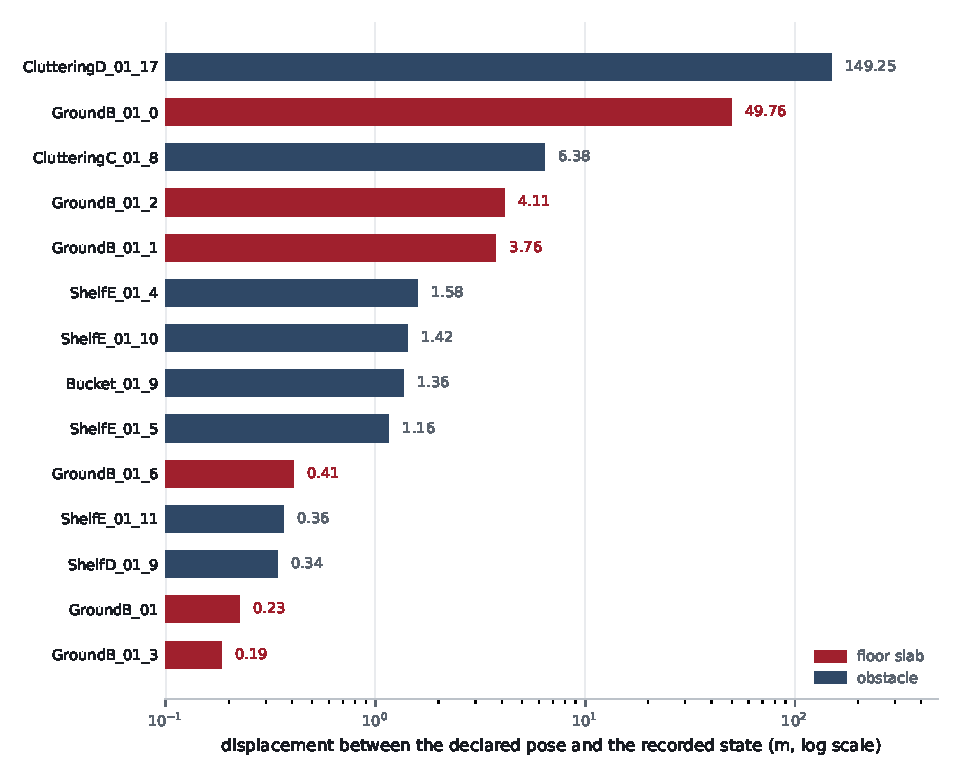
\includegraphics[width=0.86\textwidth]{figures/state_drift.pdf}
\caption{Displacement between the declared pose of a model and the pose
recorded in the world's saved state, for the fourteen models at which the two
disagree. Logarithmic axis; the discrepancies span three orders of magnitude.
Five of the fourteen are floor slabs, so the correction alters the extent of
the floor and not only the placement of obstacles upon it.}
\label{fig:drift}
\end{figure}

The consequence is that a floor plan rasterised from the declarations describes
a building the simulator does not load. Obstacles appear where the floor is
clear; floor appears where an obstacle stands; and the placement of five of the
nine floor slabs is wrong, one of them by $49.76$\,m. The failure mode this
produces in execution is a robot behaving correctly in a world of which the
planner holds an incorrect map, which admits no local diagnosis.

\subsection{Two subsidiary defects in the same reader}

Two further defects were identified in the same component and are reported here
because each is silent.

\paragraph{Malformed pose fields} Two of the recorded poses are written with
adjacent numeric fields unseparated, in the form
\code{13.8354 41.7933-0.191335}. Tokenisation on whitespace yields a field that
does not parse as a number. The conventional recovery, a \code{try}\,/\,%
\code{except} returning the origin, places a $14 \times 21$\,m floor slab at
$(0,0)$ and emits no diagnostic. Numeric fields are now extracted by regular
expression, which cannot fail in that manner.

\paragraph{Nested models} The world contains a model element named
\code{Untitled} which is a grouping construct and not an asset: it holds a
bucket and a desk, each placed relative to the group. Enumeration of the
world's direct children returns the group, whose name appears in no footprint
table, and both contained obstacles are discarded. The floor beneath them was
therefore rasterised as free, and lanes were admitted across it. Model
enumeration is now recursive, with poses composed along the nesting.

\subsection{Consequences}

Table~\ref{tab:floor} records the derived floor before and after the
correction.

\begin{table}[H]
\centering\small
\caption{The derived floor, read from the declared poses and from the poses the
simulator loads. The left column comprises the figures published in the
companion report; they are superseded by the right.}
\label{tab:floor}
\begin{tabular}{@{}lrr@{}}
\toprule
 & \textbf{Declared poses} & \textbf{Poses loaded} \\
\midrule
Obstacles                & 153    & 155    \\
Waypoints                & 261    & 289    \\
Directed lanes           & 1\,652 & 1\,870 \\
Aisle waypoints          & 35     & 39     \\
Connected components     & 1      & 1      \\
\bottomrule
\end{tabular}
\end{table}

All three chargers are displaced by the correction, one of them by eleven
metres. Spawn poses for the fleet were previously held as constants in the
launch description and agreed with the graph by inspection. A constant copied
from a superseded graph places a robot at coordinates the fleet manager does
not associate with it, and the first navigation command is then issued from a
position the robot does not occupy. Spawn poses are now read from the charger
waypoints of the graph, which removes the possibility of disagreement.

The site of the companion report does not survive the correction: on the
corrected floor no side of that waypoint admits the sensed object under the
criteria of Section~\ref{sec:sites}. The single-site mission is now configured
at \site{a17}.

%  ======================================================================
\section{Selection of sites}
\label{sec:sites}

\subsection{Criteria}
\label{sec:sitecriteria}

A survey site must satisfy three conditions simultaneously, each of which is
measurable from the collision extents of the world.

\begin{enumerate}[leftmargin=1.4em, itemsep=2pt]
  \item \textbf{The empty waypoint must read open.} The sensing action reports
        contamination when the nearest finite laser return falls below a
        threshold. A waypoint with structure within that threshold reports
        contamination in every world, including those containing no sensed
        object, and the sensing action degenerates to a constant.
  \item \textbf{The sensed object must have an admissible position.} It must
        stand on floor, clear of the racks, and clear of every lane the fleet
        may traverse. The third condition is the one the companion report
        shipped without: an object placed for visual effect overlapped a
        charger lane by $0.20$\,m, and a robot was held stationary against it
        while the fleet reported its task underway, with no component reporting
        a collision.
  \item \textbf{The two readings must be separated by the threshold with
        margin.} A site at which the occupied and empty readings straddle the
        threshold by centimetres is a site whose branch is determined by the
        stopping position of the fleet.
\end{enumerate}

These are evaluated from \code{config/aws\_footprints.json}, the same footprint
table from which the navigation graph is rasterised, so the two cannot
disagree. Thirteen of the thirty-nine aisle waypoints satisfy all three.

\subsection{The three sites}

\begin{table}[H]
\centering\small
\caption{The three sites, and the admissible position of the sensed object at
each. Clearances are computed from the collision extents; the sensed object is
a $0.9 \times 0.5 \times 0.9$\,m box placed $0.80$\,m from the waypoint with
its major axis directed at it.}
\label{tab:sites}
\begin{tabular}{@{}llrlrrr@{}}
\toprule
\textbf{Site} & \textbf{Position} & \textbf{Empty} & \textbf{Side}
  & \textbf{Occupied} & \textbf{Rack} & \textbf{Lane} \\
\midrule
\site{a17} & $(1.49,\ 15.75)$   & 1.48 & west & 0.35 & 0.44 & 0.35 \\
\site{a31} & $(15.24,\ 37.00)$  & 1.24 & west & 0.35 & 0.87 & 0.35 \\
\site{a06} & $(30.24,\ -1.75)$  & 1.71 & east & 0.35 & 0.46 & 0.35 \\
\bottomrule
\end{tabular}
\end{table}

\site{a17} is a terminal waypoint: one lane enters it and that lane is the only
exit. Where a side is admitted at all it is admitted at the minimum lane
clearance of $0.35$\,m, which is the robot radius of $0.25$\,m together with a
margin of $0.10$\,m.

% Floated. Held in place it is too tall to follow the text on its page and
% leaves half of one blank.
\begin{figure}[tbp]
\centering
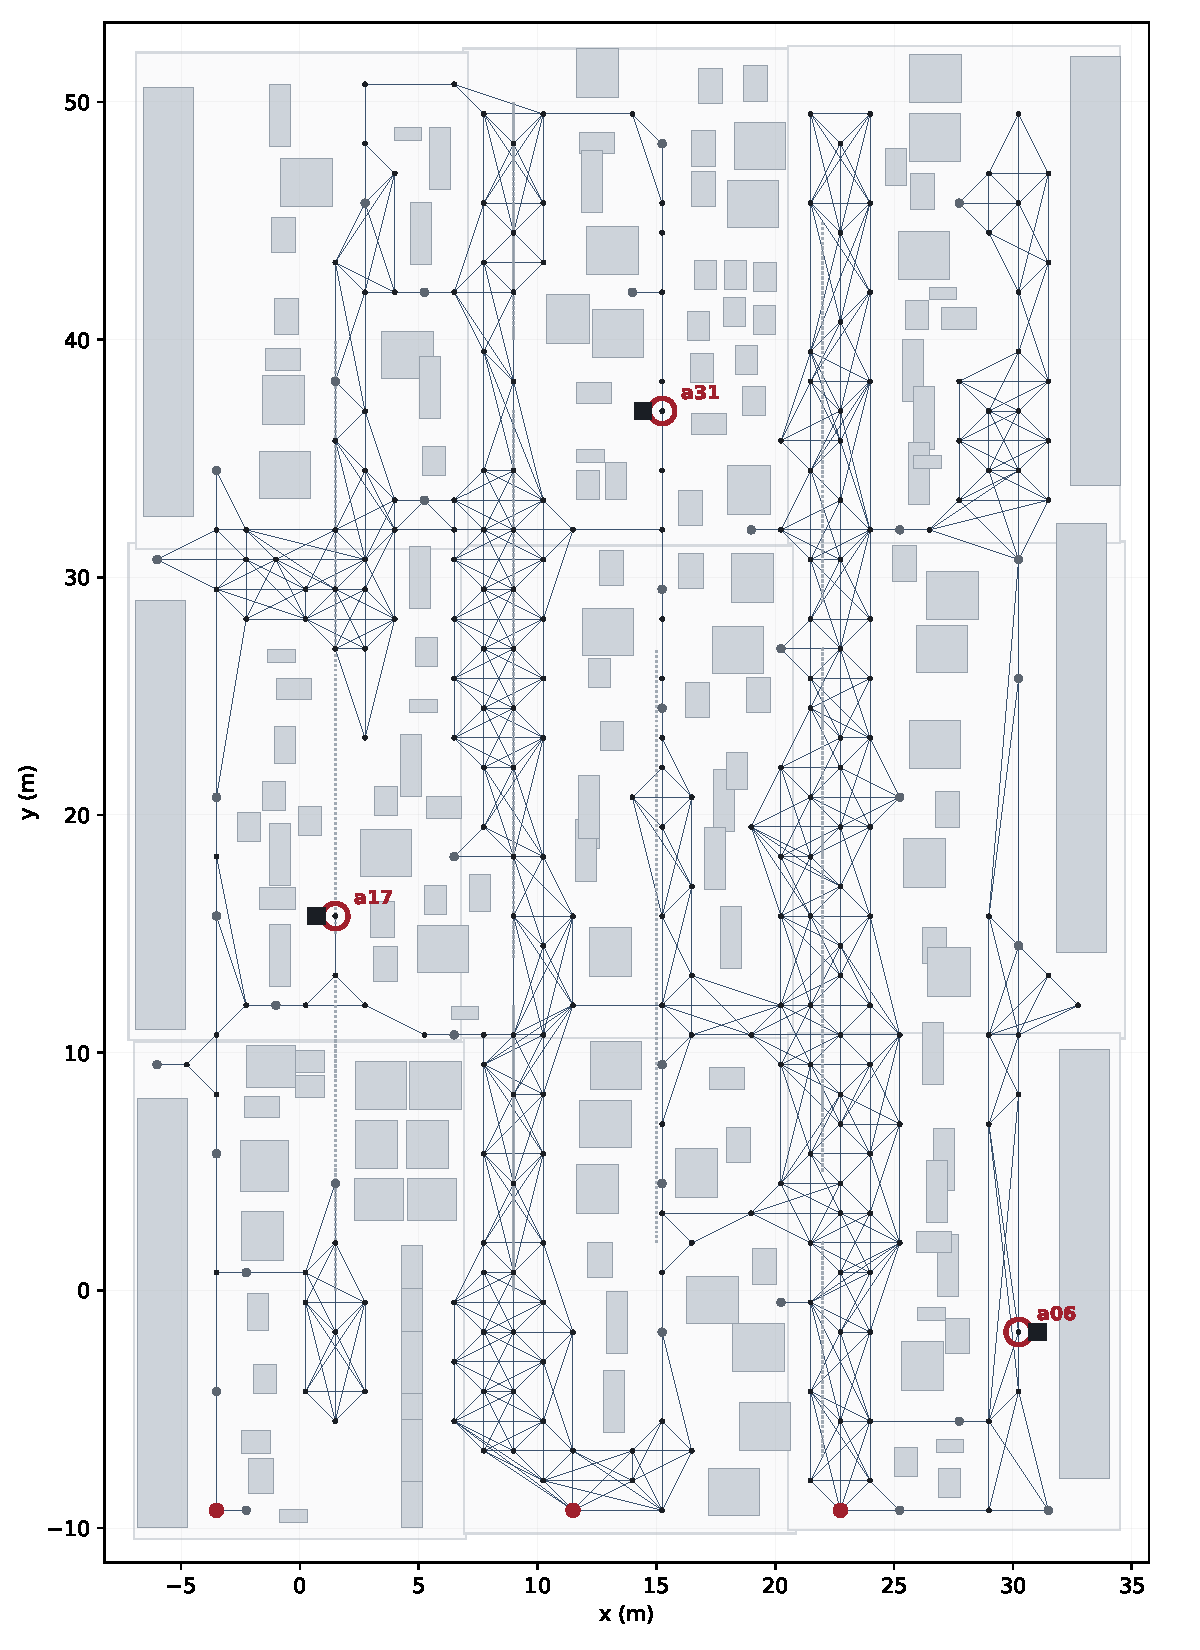
\includegraphics[width=0.66\textwidth]{figures/floor_sites.pdf}
\caption{The corrected floor and the roadmap derived from it: $289$ waypoints,
$1\,870$ directed lanes, $155$ obstacles. Obstacles are shaded; lanes are drawn
in outline; chargers are marked in red on the south wall; the three sites are
ringed and the position of the sensed object at each is marked by a filled
square. The dotted paths are the circuits of the nine scripted pedestrians,
which are excluded from the graph.}
\label{fig:floor}
\end{figure}


\subsection{The admissible sites of the floor}

Table~\ref{tab:allsites} gives every waypoint the criteria admit. Thirteen of
the thirty-nine aisle waypoints qualify, and the three of
Table~\ref{tab:sites} were selected from them on two further grounds: that the
two scanned sites be a real transit from their chargers, and that the third be
distant from both, so that a claim about a location nobody visited is not a
claim about a location adjacent to one that was.

\begin{table}[H]
\centering\small
\caption{Every waypoint admitted by the criteria of
Section~\ref{sec:sitecriteria}. The three in use are set in bold. The occupied
reading is 0.35\,m at every row, since the sensed object is placed by the same
rule at each; the lane clearance is 0.35\,m at every row, since where a side is
admitted at all it is admitted at the minimum.}
\label{tab:allsites}
\begin{tabular}{@{}llrlr@{}}
\toprule
\textbf{Waypoint} & \textbf{Position} & \textbf{Empty} & \textbf{Side}
  & \textbf{Object at} \\
\midrule
\code{aisle\_02} & $(31.49,\ -9.25)$ & 1.43 & east  & $(32.29,\ -9.25)$ \\
\code{aisle\_04} & $(-3.51,\ -4.25)$ & 1.23 & east  & $(-2.71,\ -4.25)$ \\
\code{aisle\_05} & $(15.24,\ -1.75)$ & 1.09 & west  & $(14.44,\ -1.75)$ \\
\textbf{\code{a06}} & $(30.24,\ -1.75)$ & 1.71 & east & $(31.04,\ -1.75)$ \\
\code{aisle\_12} & $(-6.01,\ 9.50)$  & 1.43 & south & $(-6.01,\ 8.70)$ \\
\textbf{\code{a17}} & $(1.49,\ 15.75)$ & 1.48 & west & $(0.69,\ 15.75)$ \\
\code{aisle\_19} & $(6.49,\ 18.25)$  & 1.00 & west  & $(5.69,\ 18.25)$ \\
\code{aisle\_21} & $(25.24,\ 20.75)$ & 1.28 & east  & $(26.04,\ 20.75)$ \\
\code{aisle\_22} & $(15.24,\ 24.50)$ & 0.97 & west  & $(14.44,\ 24.50)$ \\
\code{aisle\_23} & $(30.24,\ 25.75)$ & 1.58 & east  & $(31.04,\ 25.75)$ \\
\code{aisle\_31} & $(-3.51,\ 34.50)$ & 0.98 & north & $(-3.51,\ 35.30)$ \\
\textbf{\code{a31}} & $(15.24,\ 37.00)$ & 1.24 & west & $(14.44,\ 37.00)$ \\
\code{aisle\_34} & $(5.24,\ 42.00)$  & 1.17 & south & $(5.24,\ 41.20)$ \\
\bottomrule
\end{tabular}
\end{table}

Two features of the table bear on the criteria that produced it. The empty
reading ranges from 0.97 to 1.71\,m, so every admitted waypoint clears the
threshold by at least $0.27$\,m and the margin of Section~\ref{sec:sitecriteria}
is not the binding constraint at any of them. And the side admitted is
determined by the racks and is not free: of the fifty-two candidate placements
these thirteen waypoints offer, thirteen are admitted, so no waypoint here
admits its object on more than one side except \code{a17}, whose aisle is
wide enough for three.

\subsection{Agreement between the model and the sensor}

The analytic criteria admit direct comparison against the simulator, and the
agreement is not uniform. Two regimes are distinguished.

The predicted reading for the occupied case is reliable. The criteria give
$0.35$\,m for the nearest face of the sensed object, against measurements of
$0.32$--$0.34$\,m in the companion report and $0.33$--$0.41$\,m in the runs of
Section~\ref{sec:runs}. The object is a box whose vertical extent the model and
the sensor agree upon.

The predicted reading for the empty case is not reliable. The criteria give
$1.71$\,m at \site{a06} where the sensor returned $2.25$\,m, and $1.48$\,m at
\site{a17} where the sensor returned $0.97$ and $1.08$\,m. Two causes account
for the discrepancy in both directions. The criteria are two-dimensional and
the sensor is a plane at $0.26$\,m above the floor, so structure shorter than
that plane is an obstacle to the former and invisible to the latter. And the
nine pedestrians are excluded from the criteria by construction and are
entirely visible to the sensor.

The criteria are therefore serviceable for refusing a site and are not
serviceable for predicting a reading. Every admitted site carries in excess of
one metre of clearance, and that margin absorbs the half metre of disagreement
observed.

%  ======================================================================
\section{Execution}
\label{sec:execution}

\subsection{The chain from domain to floor}
\label{sec:chain}

Figure~\ref{fig:chain} gives the components between an \textsc{epddl} domain
and a robot on a floor, and the interface at which each defect of
Section~\ref{sec:defects} was found. The chain is stated because the failures
reported below are properties of the interfaces and not of the components, and
the interfaces are not otherwise visible.

\begin{figure}[H]
\centering
\begin{tikzpicture}[
  x=1mm, y=1mm,
  comp/.style={draw=ink, fill=mist, rounded corners=1.5pt, inner sep=2.5pt,
               font=\scriptsize, align=center, minimum width=26mm,
               minimum height=8mm},
  art/.style={draw=rulegrey, fill=white, inner sep=2.5pt,
              font=\ttfamily\tiny, align=center, minimum width=24mm,
              minimum height=7mm},
  ep/.style={comp, draw=signal},
  flow/.style={->, >=Latex, draw=slate, line width=0.5pt},
  side/.style={->, >=Latex, draw=signal, line width=0.5pt, dashed},
  note/.style={font=\tiny, text=slate, align=center}]

  % --- offline: domain to policy
  \node[art]  (dom)  at (  0,   0) {domain.epddl\\problem.epddl};
  \node[comp] (gr)   at ( 33,   0) {\code{plank}\\grounder};
  \node[art]  (task) at ( 66,   0) {ground task\\12 atoms, 3 worlds};
  \node[ep]   (sol)  at ( 99,   0) {\code{EpistemicPlanSolver}\\AO$^*$};
  \node[art]  (pol)  at (132,   0) {policy\\8 nodes, 3 leaves};
  \foreach \a/\b in {dom/gr, gr/task, task/sol, sol/pol} \draw[flow] (\a) -- (\b);

  % --- online: policy to floor
  \node[comp] (exe) at (132, -26) {\code{executor}\\behaviour tree};
  \node[ep]   (st)  at ( 99, -26) {\code{epistemic\_state}\\product update};
  \node[comp] (br)  at ( 99, -47) {\code{eplansys\_rmf\_bridge}\\action performers};
  \node[comp] (rmf) at ( 53, -47) {Open-RMF\\adapter, schedule};
  \node[comp] (gz)  at (  7, -47) {Gazebo\\\code{slotcar}, laser};
  \node[ep]   (per) at ( 53, -68) {\code{site\_perception}\\threshold on \code{/rN/scan}};

  \draw[flow] (pol) -- (exe);
  \draw[flow] (exe) -- (st);
  \draw[flow] (exe.south) -- ++(0,-11) -| (br.east);
  \draw[flow] (br) -- (rmf);
  \draw[flow] (rmf) -- (gz);
  \draw[side] (gz.south) |- (per.west);
  \draw[side] (per.east) -| (br.south);
  \node[note] at (78, -60) {\code{<place> <outcome>}};
  \draw[flow] (br.north) -- ++(0,7) -| (st.south);

  % --- the floor the other two rows are defined over
  \node[art]  (wor) at (  7, -90) {\code{warehouse.world}};
  \node[ep]   (rw)  at ( 53, -90) {\code{read\_world.py}\\rasterise, thin};
  \node[art]  (nav) at ( 99, -90) {nav graph\\289 waypoints};
  \draw[flow] (wor) -- (rw);
  \draw[flow] (rw) -- (nav);
  % Left of the bridge and right of the perception node, which is the
  % only clear column between the two rows.
  \draw[flow] (nav.west) -- ++(-8,0) |- (rmf.east);
  \draw[flow] (wor.north) -- (gz.south);

  \node[note, anchor=north west, align=left] at (-14, -101)
    {Red outline: a component holding or producing epistemic content.\\
     Dashed: an observation.};
\end{tikzpicture}
\caption{The chain from an \textsc{epddl} domain to a robot on a floor. The
upper row is offline and runs once per problem; the middle rows execute the
policy the upper row returned; the lower row derives the floor both the fleet
and the planner's site names are defined over. Every defect of
Section~\ref{sec:defects} lies on an arrow of this figure and none within a
box.}
\label{fig:chain}
\end{figure}

Four of the eight defects lie on the arrows of the lower row, which is the
derivation of the floor: the state block, the malformed poses and the nested
models are all read errors at
\code{warehouse.world} $\to$ \code{read\_world.py}, and the charger
displacement is a disagreement between the graph that arrow produces and a
constant held elsewhere. Two lie between \code{site\_perception} and the
bridge, which is the attribution of an observation to an action. One lies
between the solver and the executor, where the search occupies a process the
bringup also needs. One lies between the four files that name the sites, which
is an interface with no arrow in the figure at all, and that is why it went
unchecked.

\subsection{The correspondence between the two halves}
\label{sec:mapping}

The executor drives a behaviour tree over a classical \textsc{pddl} domain and
the policy is a tree over an \textsc{epddl} one. The two are joined by a table
mapping each grounded epistemic action onto a grounded classical action and a
duration. The table is not a translation: it is a modelling decision, it is
stated here, and Section~\ref{sec:defectclass} records that it is the one
interface of the system for which no mechanical check exists.

The domain grounds $72$ epistemic actions over three agents and three sites:
nine \code{goto}, nine \code{scan}, and $54$ announcements, being two
announcement types over every $(\text{speaker}, \text{listener}, \text{site})$
triple. The drafting tool resolves the first $18$, whose names it finds in the
classical domain, and declines the remaining $54$.

The refusal is correct and its ground is the design of the domain. There is no
\code{relay-dirty} in the classical half and there cannot be one. That half is
deliberately blind to the content of an utterance, and a classical planner able
to distinguish the report of contamination from the report of its absence would
be reasoning about the proposition the epistemic half exists to reason about.
The correspondence is therefore not derivable from the two domains, and a tool
that inferred one would be inventing it.

The decision, once taken, is a single rule. Both announcements carry the same
classical content, namely that one agent addressed another about a site, and
both are therefore sent to the same classical
\code{(relay ?i ?j ?s)}. What distinguishes them is the world the speaker
occupied when speaking, which is precisely what the epistemic model holds and
the classical domain does not represent.

\begin{align*}
\code{relay-dirty\_}i\code{\_}j\code{\_}s \;&\longmapsto\;
  \code{(relay }i\ j\ s\code{)}, \quad 2.0\,\mathrm{s} \\
\code{relay-clean\_}i\code{\_}j\code{\_}s \;&\longmapsto\;
  \code{(relay }i\ j\ s\code{)}, \quad 2.0\,\mathrm{s}
\end{align*}

The map is not injective, and the loss of information is deliberate and exactly
located: the fibre over each classical \code{relay} has two elements, and which
of the two was executed is recoverable only from the epistemic model. The
executor cannot tell them apart, which is the intended property, since the
executor's task is to move robots and hold no opinion about contamination.

Two consequences are worth stating. First, the durations differ by kind: a
\code{goto} and a \code{scan} are given $1.0$\,s and an announcement $2.0$\,s,
these being the interval the bridge holds before reporting the action done, and
not an estimate of any physical duration. Nothing moves in order to speak, so
Open-RMF is not asked for anything and the figure is a pause. Second, the
policy of Section~\ref{sec:policy} uses four of the $54$ announcements. The
other $50$ exist because the grounder is exhaustive, and their presence in the
table costs one rule to write and nothing to maintain.

The failure mode this arrangement admits is the sixth defect of
Section~\ref{sec:defects}: the classical \code{relay} carried a precondition
the epistemic \code{relay-dirty} does not entail. Because the map is many-to-one
and crosses two languages, no component holds both sides at once, and the
contradiction was observable only by running the branch on which it bites.

\subsection{Two sensors}

The companion report fits a laser to one robot and records the reason: Gazebo
Classic derives the name of a plugin's node from the plugin, so several robots
instantiated from one model description yield several nodes of one name, and
the server terminates. With a single sensing agent the restriction is without
cost.

The three-site plan executes sensing actions at two sites with two robots, and
the restriction is therefore binding. The ray plugin accepts a ROS namespace,
and a namespace is the scope within which a node name is unique. A copy of the
laser-bearing model description is generated per sensing robot at launch, with
the plugin placed in that robot's namespace; scan topics are consequently
\code{/r1/scan} and \code{/r2/scan}. Generation at launch is preferred to
checked-in copies, which would differ by one string and would diverge upon any
modification of the geometry.

\subsection{Attribution of observations}
\label{sec:attribution}

The bridge instantiates one action performer per action name, and observations
arrive on one topic. A domain with several sites therefore routes every sensing
action through one performer and one observation field. The topic is latched,
so a performer subscribing after an earlier reading receives that reading
immediately.

The consequence for a plan that dispatches two robots to two sites is severe
and is not detectable from any single component. The second robot is already
positioned at its site when the first reports, so the value available at the
second sensing action is a genuine measurement, taken by the correct sensor at
the correct place, and attributed to the wrong action. The branch is taken, the
product update is applied, the goal is checked, and the value consumed is
whichever site reported most recently.

Temporal disambiguation is inadequate, and the inadequacy is instructive. A
robot commonly arrives at its site during the \code{goto} action preceding the
scan, so the correct reading is already several seconds old when the sensing
action begins. A rule admitting only readings newer than the action discards
the correct value and falls through to the ground truth recorded in the task
map. Since the launch derives that ground truth from the same argument that
positions the sensed object, the fallback is correct, and the defect is
therefore invisible in the run.

Observations are consequently published in the form
\code{<place> <outcome>}, and the bridge resolves the entry for the place its
own action names, taken from the argument the task map declares as selecting
the outcome. Two sensing actions at two places cannot answer for one another
under any ordering in time.

\subsection{Perception}

Both sensing robots carry a planar laser on the mast at $0.33$\,m, with $180$
beams over the full revolution and returns admitted between $0.12$ and
$3.5$\,m. The perception node subscribes to the fleet state and to each robot's
own scan topic, and withholds a verdict until the fleet has reported that robot
within $0.40$\,m of a site on three consecutive reports. It then reads the
nearest finite return, compares it against $0.70$\,m, and publishes.

The node is not informed of the plan. An observation is generated by a robot
arriving at a location in possession of a sensor, and a perception component
requiring notification of the action in progress would report the plan back to
the system that issued it.

%  ======================================================================
\section{The three runs}
\label{sec:runs}

The floor is instantiated four times. The variants differ in the position of
one object and in nothing else: the same hall, the same $155$ obstacles, the
same nine pedestrians, the same navigation graph, the same binary, the same
domain, the same goal, the same threshold of $0.70$\,m.

\begin{table}[H]
\centering\small
\caption{Three worlds, three leaves. Readings are the nearest finite return
reported by the perception node at the point of the corresponding sensing
action. Checks comprise nine formulas evaluated against the epistemic state
after the fleet came to rest, and two transcripts of address.}
\label{tab:runs}
\begin{tabular}{@{}llllrl@{}}
\toprule
\textbf{Object at} & \textbf{scan \site{a17}} & \textbf{scan \site{a06}}
  & \textbf{Leaf} & \textbf{Actions} & \textbf{Checks} \\
\midrule
\site{a17} & dirty, 0.33\,m & not reached &
  \code{relay-clean\_scout\_relay\_a06} & 4 & 11 of 11 \\
\site{a06} & clean, 1.08\,m & dirty, 0.41\,m &
  \code{relay-clean\_relay\_scout\_a31} & 6 & 11 of 11 \\
\site{a31} & clean, 0.97\,m & clean, 2.25\,m &
  \code{relay-clean\_relay\_scout\_a06} & 6 & 11 of 11 \\
\bottomrule
\end{tabular}
\end{table}

The fourth variant contains no sensed object. It is a control and is excluded
from the table: the domain asserts that exactly one site is contaminated, so a
world containing no such object contradicts the problem the planner was given.

The third row is the case for which the domain exists. Both sensing actions
return \code{e-scan-clean}; no measurement is taken at \site{a31} at any point
in the run; and the team terminates in possession of
$\Kw{\mathit{scout}}\,\mathit{contaminated}(\site{a31})$ and
$\Kw{\mathit{relay}}\,\mathit{contaminated}(\site{a31})$. The models that run
passed through are given in Section~\ref{sec:updates}.

\subsection{Determinism of the epistemic trajectory}
\label{sec:determinism}

That row was executed eight times, on eight separate instantiations of the
simulator, and the seven models recorded after each product update were
compared file by file across all of them. Every one of the $56$ files agrees
with its counterpart exactly: the same worlds in the same order, the same
designated sets, the same valuations, and the same accessibility relations for
all three agents.

The comparison is worth making because the physical runs did not agree with
one another in any other respect. The pedestrians occupied different positions
throughout, the robots spent different amounts of time on the same lanes, the
runs differed in wall-clock length, and the two sensing actions returned a
different pair of distances every time. The readings at \site{a17} across the
eight runs span $0.96$ to $1.04$\,m and those at \site{a06} span $2.21$ to
$2.27$\,m. What the eight have in common is not a value but a side: every one
of the sixteen readings lies above the $0.70$\,m threshold.

What is invariant is the pair of outcomes those distances were thresholded
into. The epistemic state is a function of the sequence of events applied to
it, an event is selected by the outcome and not by the reading, and the
outcomes were \code{e-scan-clean} both times. The physical variation is
absorbed at the threshold, and everything after the threshold is arithmetic on
a finite structure.

This locates the entire stochastic content of the system at one comparison per
sensing action. It also states the precondition for the figures of
Section~\ref{sec:updates} to be figures of anything: they are properties of the
domain and the branch, and not of the run they happen to have been recorded
from. The corresponding warning is that a threshold near a reading would make
the epistemic result as noisy as the reading. Here the margins are $0.27$\,m
and $1.54$\,m, which Section~\ref{sec:sitecriteria} obtained by choosing the
sites and not by chance.

\subsection{The verdict}
\label{sec:verdict}

Eleven checks are evaluated after the fleet comes to rest. Nine interrogate the
epistemic state; two read the transcripts of the agents' radio channels.

\begin{lstlisting}
ok   (Kw scout contaminated_a06) holds
ok   (Kw scout contaminated_a17) holds
ok   (Kw scout contaminated_a31) holds
ok   (Kw relay contaminated_a06) holds
ok   (Kw relay contaminated_a17) holds
ok   (Kw relay contaminated_a31) holds
ok   (Kw observer contaminated_a06) does not hold
ok   (Kw observer contaminated_a17) does not hold
ok   (Kw observer contaminated_a31) does not hold
ok   relay was spoken to, 1 time(s)
ok   observer was spoken to by nobody
\end{lstlisting}

The two classes of check are of different evidential strength, and the second
is the weaker. A negative epistemic conjunct is satisfied by everything that
fails to occur, so a procedure consulting only the model cannot distinguish
deliberate exclusion from an absence of communication. The transcript check
addresses that gap and does not close it: it establishes that the excluded
agent was not addressed.

The transcript check is asserted over the relay alone. The relay is addressed
on every branch, the scout's announcement being the first speech act under
either outcome of the first scan; the scout is addressed on two branches of
three. A check naming both agents would constitute an assertion about which
branch was expected, and a run taking the short branch would be reported as a
failure for having been short.

%  ======================================================================
\section{Defects}
\label{sec:defects}

Eight defects were identified in bringing the three-site mission into
operation. None is an error within a component. Each is a property of the
composition, and each was unobservable while the domain carried one site and
one sensing robot. Table~\ref{tab:defects} records them.

\begin{table}[H]
\centering\small
\caption{Defects identified, with their proximate cause and classification.}
\label{tab:defects}
\begin{tabularx}{\textwidth}{@{}p{0.30\textwidth}Xl@{}}
\toprule
\textbf{Symptom} & \textbf{Cause} & \textbf{Class} \\
\midrule
The navigation graph describes a building the simulator does not load &
The world carries a saved state block which Gazebo applies over the declared
poses; fourteen disagree, one by $149$\,m &
Geometric \\
\addlinespace
A $14 \times 21$\,m floor slab is placed at the origin &
Two recorded poses have adjacent numeric fields unseparated, so whitespace
tokenisation yields a non-numeric field and the conventional recovery returns
the origin &
Parsing \\
\addlinespace
Lanes are admitted across a bucket and a desk &
Both are nested within a grouping model whose name appears in no footprint
table; enumeration of direct children discards them &
Geometric \\
\addlinespace
A valid policy is returned to a system that has terminated; the mission fails
at \code{send\_goal failed} &
The readiness test admitted a configured node, and six seconds of search
starved the lifecycle manager sharing the process &
Race \\
\addlinespace
A sensing action reports a valid measurement, taken by the correct sensor at
the correct place, for the wrong site &
One performer per action name and one latched observation topic; the second
sensing action receives the first one's value on subscription &
Composition \\
\addlinespace
One branch of three does not proceed past
\code{Error checking at start reqs} &
The classical precondition required the speaker of an announcement to have
scanned the site it names &
Modelling \\
\addlinespace
The executor reports a precondition over a non-existent object, fifty times per
second, indefinitely &
Four files name the sites and no check compared them; three were renamed and
the fourth was not &
Duplication \\
\addlinespace
The post-run check reports three formulas \code{UNCHECKED} and the mission
failed, on a run satisfying its goal &
The check component's defaults are the propositional formulas, and this domain
grounds one atom per site &
Configuration \\
\bottomrule
\end{tabularx}
\end{table}

Three warrant discussion.

\subsection{A race the small domain concealed}

The planning system is a single process, and a plan request is served on the
same executor upon which the lifecycle manager's activation calls arrive.
Solving the propositional problem requires forty expansions and returns before
the coincidence is observable. Solving the three-site problem occupies the
process for six seconds, during which the activation calls go unanswered and
the bringup reports \code{Failed to start plansys2!}. The planner subsequently
returns a valid eight-node policy to a system that has already terminated, and
the mission fails at \code{start\_plan\_execution} with \code{send\_goal
failed}, some forty log lines and several seconds removed from the cause.

The readiness test previously admitted any node that answered. A configured
node answers, several seconds before the bringup activates anything. The
mission now waits for every managed node to report the active state.

The general form is worth recording. Search time is a property of the domain.
The bringup is a property of the framework. The two interact because they share
a process, and no interface between them expresses the dependency.

\subsection{A precondition contradicting the domain}

The classical half of the mission is deliberately impoverished: it cannot
distinguish a broadcast from an encrypted relay, and it is not intended to.
It nonetheless gates the actions the executor drives, and one of its gates
encoded an assumption this domain exists to refute. The \code{relay} action
required \code{(scanned ?from ?s)}: the speaker of an announcement must have
scanned the site it names. Under the exactly-one constraint the announcement
carrying the finding names a site the speaker has not visited, which is the
result of Section~\ref{sec:elimination}.

The defect is observable on one branch of three. Where the first scan returns
clean, the announcement names the site just scanned and the precondition holds;
where it returns dirty, the announcement names a different site and the
executor does not proceed. Two of the three worlds executed to completion with
the incorrect precondition in place. The condition is now
\code{(has\_scanned ?from)}, which requires that the speaker has performed some
sensing action.

\subsection{A correct refusal}
\label{sec:refusal}

The post-run check is configured by default with the propositional formulas,
and this domain has no atom $\mathit{contaminated}$: the grounder produces one
atom per site. Presented with formulas naming an atom outside the task, the
check reported them \code{UNCHECKED} and failed the run.

That behaviour is correct and is recorded because the alternative is
consequential. A check returning \emph{false} for a formula it cannot evaluate
would report a satisfied run as unsatisfied, and, on the negative conjunct,
would report an unsatisfied run as satisfied. The distinction between
\emph{does not hold} and \emph{could not be evaluated} is load-bearing wherever
a goal contains a negative epistemic conjunct.

\subsection{One observation without explanation}

On the floor as read before the correction of Section~\ref{sec:floor}, the
scout halted $2.5$\,m short of its site, in open floor with $1.05$\,m of
clearance, and did not proceed. The behaviour reproduced across two runs at
coordinates agreeing to three decimal places. The robot's own laser reported an
object at $0.23$\,m to its rear, fixed with respect to the world: displacing
the robot by $0.86$\,m displaced the reading by $0.85$\,m at the same bearing.
No model in the world file, at any nesting depth, under either the declared or
the recorded poses, and no pedestrian on any leg of its circuit, lies within
$1.9$\,m of that point. The fleet manager reported the robot $10.5$\,s from its
destination for four minutes.

The behaviour has not recurred on the corrected floor and is not explained. It
is recorded because a halt presenting as a task permanently underway, with no
component reporting an error, is the signature of the class of defect this
section is concerned with.

\subsection{A characterisation of the class}
\label{sec:defectclass}

The eight defects have a property in common, and it is worth stating precisely
because it determines what would have caught them.

\begin{definition}[Locally invisible]
\label{def:invisible}
A defect is \emph{locally invisible} when the execution in which it occurs
violates no postcondition of any single component: each component receives
input satisfying its precondition, produces output satisfying its
postcondition, and reports no error.
\end{definition}

Every defect in Table~\ref{tab:defects} is locally invisible under
Definition~\ref{def:invisible}, and the consequence is that no component could
have detected any of them.

Consider the third row. \code{read\_world.py} is handed a well-formed world
file and returns a set of boxes; each box corresponds to a model it found; it
found every model it enumerated. Its postcondition is satisfied. The graph
generator is handed those boxes and returns a connected graph over the free
space they leave; its postcondition is satisfied. The fleet adapter is handed a
valid graph and routes over it; its postcondition is satisfied. A robot then
drives through a desk, and the first component in a position to observe the
discrepancy is the physics engine, which is not asked and does not report.

The same account applies to the others. In the fifth row the value the bridge
consumes is a real reading from a real sensor at a real place, so no component
holds a datum it should not. In the seventh the executor evaluates a
precondition over a term the problem does not contain and reports the failure
faithfully, fifty times a second, without the vocabulary to say that the term
is not an object of the problem. In the first the world file and the simulator
agree with each other completely; the disagreement is with a third party that
read the file differently.

\begin{table}[H]
\centering\small
\caption{What would have detected each defect. The final column names an
invariant spanning two components; none of them is expressible within one.}
\label{tab:detect}
\begin{tabularx}{\textwidth}{@{}p{0.24\textwidth}X@{}}
\toprule
\textbf{Defect} & \textbf{The invariant that would have caught it} \\
\midrule
State block &
The set of poses the rasteriser reads equals the set the simulator loads. \\
\addlinespace
Malformed pose &
Every pose field parsed yields six numbers; a field that does not is an error
and not a default. \\
\addlinespace
Nested models &
The count of models enumerated equals the count the file contains at every
depth. \\
\addlinespace
Bringup race &
No request is issued to a managed node before that node reports the active
state. \\
\addlinespace
Observation attribution &
The place at which a reading was taken equals the place the consuming action
names. \\
\addlinespace
Relay precondition &
The classical precondition of an action is implied by the epistemic
precondition of the action it stands for. \\
\addlinespace
Site name drift &
The set of sites each of the four files names is the same set. \\
\addlinespace
Check formulas &
Every atom named in a checked formula is an atom of the loaded task. \\
\bottomrule
\end{tabularx}
\end{table}

Six of the eight invariants of Table~\ref{tab:detect} are now checked, and the
two that are not are recorded as such. The site-name invariant is enforced at
launch, and the launch refuses to start when it fails. The atom invariant is
enforced by the check component, which reports \code{UNCHECKED} and was already
correct. The parse invariant is enforced by construction, since the numeric
fields are now extracted by a pattern that matches numbers. The nesting
invariant is enforced by recursion. The activation invariant is enforced by
the mission. The attribution invariant is enforced by the bridge.

The two that remain are the first and the sixth. Equality between the poses a
reader takes and the poses the simulator loads is checked for the state block
and is not checked in general, since a world file admits other constructions
that shift a pose and this correction addresses one of them. And the
implication between a classical precondition and the epistemic precondition it
stands for is not mechanically checkable at present: the two are written in
different languages over different vocabularies, and the correspondence between
them is the modelling decision of Section~\ref{sec:mapping}.

\subsection{Silent recovery as a failure mode}
\label{sec:silent}

Two of the eight arise from error handling and warrant separate treatment,
because in each the code that produced the failure was written to prevent one.

The malformed pose is the clearer case. A field that does not parse as a number
is an unambiguous signal that the reader's assumption about the file is wrong.
Converting that signal into the origin substitutes a plausible value for an
impossible one, and a plausible value propagates: a floor slab at $(0,0)$
overlaps eight others, the union is still a floor, the graph over it is still
connected, and nothing downstream has grounds to object. An exception at the
point of the parse would have been reported with the field in hand.

The second is the argparse failure, which is the same shape inverted. The
option \code{-{}-pallet} followed by \code{-4.15,2.0,0} is rejected with
\code{expected one argument}, which names the option and not the value, and
the value is what is wrong with it. The recovery here is the reader's: the
message is accurate and its subject is misleading, and a message naming the
token it declined to accept would have been read correctly the first time.

The general form is that a recovery is safe exactly when the recovered value is
distinguishable from a legitimate one. The origin is not distinguishable from a
legitimate pose. \code{UNCHECKED} is distinguishable from \emph{false}, which
is why the check component of Section~\ref{sec:refusal} is correct and these
two are not.

%  ======================================================================
\section{The recording}
\label{sec:recording}

The run is filmed, and the apparatus is described here because two parts of it
had to be built and one of those exists to work around a defect in a tool.

\subsection{The display}

The capture is a $3840 \times 1080$ grab of an X server with no physical
device behind it, carrying the simulator and the visualiser and nothing else.
A grab of the real desktop would pick up whatever else were open on it, and a
figure that shows a terminal window is a figure that has to be cropped by hand
every time it is regenerated.

There is no window manager on that display, and the consequence is not
cosmetic. A request to resize a window is granted by the X server and never
reaches the toolkit, which does not relay out, so both windows are positioned
and sized before they map: the simulator from its own preferences file, which
it reads once at startup and offers no command line for, and the visualiser
from the configuration this package already ships.

\subsection{The camera follows the robot}

A fixed camera does not serve this run. The scout crosses some forty metres of
warehouse, and the aisle it arrives at is one frame of that journey; a camera
placed to frame the arrival shows an empty aisle for eight minutes first.

Gazebo Classic offers three ways to move the view and two of them do not
apply. The pose in \code{<gui><camera>} is read once at load. A
\code{<track\_visual>} element naming a model can only name one that exists at
load, and the robots are spawned some forty seconds later by a timer.

The third is the command \code{gz camera -c user\_camera -f r2}, which is
documented to follow a model and which does not work here. It advertises on
\code{\textasciitilde/user\_camera/cmd} and calls
\code{WaitForConnection} before publishing. Nothing subscribes to that topic:
it is a camera-sensor topic and the graphical client's view camera is not a
camera sensor. The command therefore blocks indefinitely, and the first
recording attempt made with it produced no film at all, because the script that
called it never reached the line that starts the capture.

\begin{table}[H]
\centering\small
\caption{The failure of \code{gz camera} against
Definition~\ref{def:invisible} and the account of
Section~\ref{sec:silent}. It is the pure case: the recovery is not a wrong
value but no value, held indefinitely.}
\label{tab:gzcamera}
\begin{tabularx}{\textwidth}{@{}p{0.26\textwidth}X@{}}
\toprule
\textbf{Component} & \textbf{What it did} \\
\midrule
\code{gz camera} &
Advertised the topic it was asked to, and waited for the subscriber its
protocol requires. Its postcondition is not violated; it is not reached. \\
\addlinespace
The client's view camera &
Subscribed to the topics it owns. It does not own that one, and is not
required to. \\
\addlinespace
The recording script &
Called a command that returns, and waited. Nothing reported an error, and the
capture that should have started did not. \\
\bottomrule
\end{tabularx}
\end{table}

The distinguishability criterion of Section~\ref{sec:silent} applies directly.
A command that cannot reach its subscriber and says so is distinguishable from
one that succeeded; a command that blocks is not distinguishable from one that
is merely slow, and a caller has no way to choose a timeout that is right for
both.

What the view camera does subscribe to is
\code{\textasciitilde/user\_camera/joy\_pose}, which sets its pose outright.
The camera is therefore driven by a component of this package,
\code{chase\_camera}, which subscribes to the simulator's own pose stream,
takes the pose of the named robot, computes where a camera trailing it should
be, and publishes that. It speaks Gazebo transport and no \textsc{ros}: a
component that tells the simulator where to point a camera has no place on the
robot's control graph, and putting it there would make the recording a
dependency of the mission.

Two properties of the filter are worth stating, since neither is optional and
both are invisible when correct.

\paragraph{The pose is filtered and not followed} The camera trails the robot
along the robot's own heading. Taking that heading directly puts the camera
through every rotation the robot makes, and this robot turns in place at every
waypoint; the result is a film in which the warehouse rotates about a
stationary robot. The target pose is approached through a first-order filter
with a time constant of $0.45$\,s, so the robot turns within the frame and the
camera comes round after it. The filter coefficient is computed from the
interval between messages and not fixed per message. The simulator's
real-time factor moves whenever a robot comes into another's view, and a fixed
coefficient would make the camera lag by an amount that depends on the
scene.

\paragraph{Yaw is interpolated on the circle} Blending $179^\circ$ towards
$-179^\circ$ on the line gives $358^\circ$ of rotation for a robot that
turned through two, and the camera swings the whole way round to arrive where
it began. The difference is wrapped into $(-\pi, \pi]$ before it is scaled.

\paragraph{The filter runs on a clock and not on the pose stream} This is the
substantive correction, and the recording that exposed it looked like a
tracking failure of the ordinary kind. At the moment the scout arrived at its
site, the camera stopped several metres short and pointing at the wrong part of
the aisle, and the robot was a speck in the corner of the shot for the whole
epistemic sequence, which is the part of the film the rest of it exists to
reach.

The cause is a property of the simulator's pose stream and not of the filter.
Gazebo publishes \code{\textasciitilde/pose/info} for models whose pose has
changed. A robot that stops therefore leaves the stream, and a camera stepped
once per message stops with it, wherever it had got to. A robot stops by
turning in place to face its site, which is the point on the trajectory at
which the camera is furthest from its target, so the view froze mid-swing. The
callback now records the robot's pose and nothing else, and the filter steps
$25$ times a second whether a message arrived or not. A stationary robot is
exactly the case in which a settled shot is wanted, and it was the only case
the first version could not produce.

\paragraph{The camera trails the direction of travel and not the heading} This
is the second correction, and it is geometric.

An aisle is a corridor, and a robot arrives at a site by driving down the
corridor and then turning in place to face the site. Two and a half metres
behind a robot that has just turned through ninety degrees is inside the rack
it turned to face. A camera trailing the robot's heading walks into that rack
over the following second, and the recording made that way shows the aisle from
inside a pallet for the whole epistemic sequence.

Slowing the filter on the heading does not fix this, and the reason is worth
stating because it was the first thing tried. The robot stands at its site for
the whole sequence, so a filter on the heading, at any time constant, converges
during exactly the part of the run the film exists for. Delaying an arrival at
the wrong place is not a correction.

The direction of travel does not have the defect. It is undefined while the
robot is stopped, and holding the last value is the right thing to do with it:
the robot drove through that space to arrive, so there is nothing in it. The
velocity is filtered before the direction is taken from it, because a robot
turning in place creeps a few millimetres per step and the direction of a creep
is noise; below $0.08$\,m\,s$^{-1}$ the direction is not updated at all.

\begin{table}[H]
\centering\small
\caption{The three corrections to the camera, and what each recording showed
before it. None of the three is visible in a still frame: each produces a
recording in which the simulator, the fleet and the mission are all behaving
correctly and the camera is looking at the wrong thing.}
\label{tab:camera}
\begin{tabularx}{\textwidth}{@{}p{0.28\textwidth}X@{}}
\toprule
\textbf{Correction} & \textbf{What the recording showed without it} \\
\midrule
Step on a clock, not on the pose stream &
The camera stops when the robot stops, since a stationary model leaves
\code{\textasciitilde/pose/info}. The robot stops by turning in place, which is
where the camera is furthest from its target, so the view froze mid-swing. \\
\addlinespace
Trail the direction of travel, not the heading &
The camera converges to a point inside the rack the robot turned to face, and
holds it for the whole of the sensing, the announcement and the verdict. \\
\addlinespace
Publish at a fixed rate, and log where nothing overwrites it &
The process did not survive a full run at the pose stream's rate, and its exit
was overwritten in the run log by the launch, which held the same file at a
fixed offset. \\
\bottomrule
\end{tabularx}
\end{table}

\paragraph{The camera has to outlive the run, and say if it does not} An
earlier recording came out as an eight-minute shot of an aisle the robot had
left in the sixth minute: the process driving the camera exited, the view held
its last pose, and the robot drove away from it. Publishing one camera pose per
message on a stream carrying every model in the world was some twenty times
more traffic than the fixed rate now produces, and the process did not survive
a whole run of it.

Nothing reported the exit, and the reason is the second half of the defect. The
camera's output was appended to the run log, which the launch held open at a
fixed offset; the launch's next write overwrote it. The camera now writes to a
file nothing else holds, the pose callback does not let an exception escape
onto the transport thread, and a supervisor restarts the process if it exits. A
restart costs one visible jump of the view, and replaces a film of an empty
aisle.

This is the third instance in this report of one shape, after the pose
defaulted to the origin and the option that named itself instead of its
argument. A component stopped; what made the stop expensive is that the record
of it was destroyed by an unrelated component holding the same file.

\subsection{The captions and the cards}

Captions are matched against the mission's own log and timed by the
\textsc{ros} timestamp of the line that carries them, offset against the moment
the capture opened and divided by the playback speed of the segment they fall
in. A caption saying that a robot sensed something appears at the frame in
which it did. The alternative, timing captions by hand against a recording, is
how a film comes to assert what the run did not do; and it would not survive
this domain in any case, since which site is scanned second, and whether it is
scanned at all, depends on what the first laser returned.

The film opens and closes on a card, and the closing card carries the one thing
the footage cannot. The site the team ends up knowing about is the site nobody
visited, so the frame in which the mission succeeds is indistinguishable from
the frame before it. Both cards are drawn from the run's own log and are not
written into the script: a card naming \site{a31} over a run that found
\site{a06} would be the single assertion in this repository a viewer has no
way to check.

%  ======================================================================
\section{What the runs establish, and what they do not}
\label{sec:established}

\subsection{Established}

Each proposition is stated existentially: there exists a run in which it held.

\paragraph{Knowledge without observation} A team terminated in possession of
the state of a site that no member visited and no sensor measured. Both sensing
actions returned clean, the third site was determined by the exactly-one
constraint, and the derived finding was transmitted on the private channel.
The negative conjunct held over that site, verified against the model and
against the transcript.

\paragraph{Two sensing agents on a derived roadmap} Two robots each contributed
one measurement, at sites $33.7$\,m apart, at transit costs of $36.5$ and
$26.8$\,m from their chargers. The selection of sites to inspect, and their
order, is determined by the planner, and the sites are separated by transits on
a graph derived from the world. This constitutes the coupling between floor and
epistemics that the companion report states it does not possess.

\paragraph{Three leaves of one policy} One conditional plan traversed three
distinct leaves in three worlds differing by the position of one object, and
satisfied its goal on each. A conditional plan reaching its goal on every
branch is the object of planning under partial observability, and is not
demonstrated by a run traversing one branch.

\paragraph{A floor derived from the poses in use} The correction of
Section~\ref{sec:floor} is established, in the sense that the figures of
Table~\ref{tab:floor} are derived from the poses the simulator applies.

\subsection{Not established}

\paragraph{Concurrency} The executor traverses a plan in strict order, so the
relay's transit completes before the scout's begins. Two agents performing
physical work is not two agents working simultaneously, and no element of this
configuration forces two robots into one corridor at one time. The
instrumentation exists; the experiment does not.

\paragraph{Scaling} Three sites is one measurement. Four sites is unsolved
within an hour of budget. What is measured is the cost of the third site, and
not a curve.

\paragraph{Object recognition} The perception component compares the nearest
finite return of a planar scan against a distance selected for these sites. It
establishes that an object is proximate to the robot at a waypoint at which, in
the empty variant, no object is. It does not identify the object.

\paragraph{Navigation among moving obstacles} The nine pedestrians traverse
fixed circuits and are absent from the navigation graph. The fleet neither
perceives nor avoids them.

\paragraph{Confidentiality} The private channel is realised by addressing, and
any node may subscribe to any topic. The available claim is that the team used
a channel on which the excluded agent was not addressed. The stronger claim
requires DDS partitions or SROS\,2 permissions, which would be constructed from
these same declared audiences; what separates the two is enforcement.

\paragraph{Completeness of the floor correction} It is established that the
declared poses are not the poses applied. It is not established that no further
discrepancy of the same kind remains, and one halt on the superseded floor is
unexplained.

%  ======================================================================
\section*{Reproduction}
\addcontentsline{toc}{section}{Reproduction}

\begin{lstlisting}
bash tools/make_site_worlds.sh /tmp
ros2 launch warehouse_xl_rmf_demo survey_sites_launch.py \
     contaminated:=a31 world:=/tmp/warehouse_xl_a31.world

python3 tools/check_sites.py                      # every admissible site
python3 tools/plot_state_drift.py --out drift.pdf # the pose disagreement
\end{lstlisting}

\noindent
\code{contaminated:=} selects the variant, and admits \site{a17}, \site{a31},
\site{a06} and \code{none}. \code{plan\_only:=true rmf:=false} returns the plan
without a simulator. Sites are read from the \textsc{epddl} problem by the
mission component and are checked against the launch description at startup,
so the four files naming them cannot diverge without refusal.

\end{document}
